\documentclass[english]{beamer}
\usetheme{JuanLesPins}
\usepackage{graphicx, tikz, bm, amsmath, mathtools, arydshln, annotate-equations, caption, wasysym, hyperref, xcolor} 
\usepackage[style=authoryear, backend=biber]{biblatex}
\addbibresource{./references/references.bib} 
\graphicspath{{./images/}}
\pgfkeys{/eqnannotate/label right/.code=\text{}}
\captionsetup[figure]{labelformat=empty}
\newcommand{\alertblue}[1]{{\color{blue}#1}}
\newcommand{\alertgreen}[1]{{\color{green}#1}}
\usetikzlibrary{positioning, tikzmark}
\usecolortheme{seahorse}
\setbeamercolor{alerted text}{fg=blue}
%------------------------------------------------
\setbeamertemplate{headline}{
  \begin{beamercolorbox}[wd=\paperwidth,ht=2.5ex,dp=1.125ex]{title in head/foot}
    \usebeamerfont{title in head/foot}\textbf{\insertshorttitle}
  \end{beamercolorbox}
  \begin{beamercolorbox}[wd=\paperwidth,ht=2ex,dp=1ex]{section in head/foot}
    \hspace*{1em} 
    \textbf{\insertsectionnavigationhorizontal{\paperwidth}{}{}} 
  \end{beamercolorbox}
}
%------------------------------------------------
\title{Distributed Lag Non-linear Models (DLNMs)}
\subtitle{Methodology and Application to Time Series Data Analysis }
\author{Vincent Arumadri}
\institute{Department of Public Health \\
\vspace{0.3cm} Erasmus MC}
\date{8\textsuperscript{th} April, 2025}
\logo{
\includegraphics[height=1.5cm, keepaspectratio]{logo-erasmusmc-2pms-wit-uk.jpg}}
\setbeamertemplate{footline}{
    \begin{beamercolorbox}[wd=\paperwidth,ht=0.3cm,dp=0.2cm]{palette primary}
        \hbox{
            \hspace{0.5cm} 
            \makebox[0.3\paperwidth][l]{\textbf{\color{white} \insertshortauthor}} 
            \makebox[0.4\paperwidth][c]{\textbf{\insertshortinstitute}} 
            \makebox[0.3\paperwidth][r]{\textbf{\insertframenumber \hspace{1cm}}}
        }
    \end{beamercolorbox}
}
\definecolor{darkblue1}{RGB}{25,25,112}
\definecolor{darkblue2}{RGB}{15,15,90}
\setbeamercolor{palette primary}{bg=darkblue1,fg=white}
\setbeamercolor{palette secondary}{bg=darkblue1,fg=white}
\setbeamercolor{palette tertiary}{bg=darkblue1,fg=white}
%------------------------------------------------
\begin{document}
%------------------------------------------------
\begin{frame}
    \titlepage
\end{frame}
%------------------------------------------------
\section{Introduction}
\begin{frame}{Key definitions}
   \begin{itemize}
    \item \alertblue{Non-linear data structure}: data where there is no linear relationship between a dependent (\alertblue{outcome/response}) and an independent (\alertblue{exposure/predictor}) variable
    \item \alertblue{Time series data}: a \alertblue{sequence of data points collected over an interval of time} e.g daily rainfall measurements, weekly sales 
    \item \alertblue{Lag}: time difference between two observations in a sequence, or the \alertblue{number of steps back in time (delay) a past observation is from the current time}
    \end{itemize}
    \vspace{0.15cm}
    \centering
    \footnotesize
    \[\begin{array}{|c|c|c|c|}
    {Day} & {Value} & {Lag-1} & {Lag-2}\\ \hline
    1 & 10 & NA & NA \\
    2 & 20 & 10 & NA \\
    3 & 30 & 20 & 10 \\
    4 & 40 & 30 & 20 \\
    5 & 50 & 40 & 30 
\end{array}\] 
\end{frame}
%------------------------------------------------
\begin{frame}{Key definitions}
    \begin{itemize}
        \item \alertblue{Autoregressive model}: specifies that the \alertblue{response} variable depends linearly on its own previous (\alertblue{lagged}) value(s)
        \begin{equation*}
            \eqnmark[blue]{node1}{y_t}=
            \eqnmark[red]{node2}{\beta_0} +
            \eqnmarkbox[blue]{node3}{\beta_2 y_{t - 1}} + 
            \eqnmark[orange]{node4}{\epsilon}
        \end{equation*}
        \annotate[yshift=-0.4em]{below, left}{node1}{Response variable}
        \annotate[yshift=-0.4em]{below, right}{node3}{Lagged response variable as predictor}
        \vspace{0.3cm}
        \item \alertblue{Distributed lag model}: specifies that the \alertblue{response} variable depends linearly on the current and (\alertblue{delayed}) lagged value(s) of predictor variables and \alert {no lagged response variables} 
        \begin{equation*}
            \eqnmark[blue]{node1}{y_t}=
            \eqnmark[red]{node2}{\beta_0} +
            \eqnmarkbox[purple]{node3}{\beta_1 x_t} + 
            \eqnmarkbox[blue]{node4}{\beta_2 x_{t-1}} + 
            \eqnmark[orange]{node5}{\epsilon}
        \end{equation*}
        \annotate[yshift=-0.4em]{below, right}{node4}{Lagged predictor}
        \annotate[yshift=-0.4em]{below, left}{node3}{Current predictor}
    \end{itemize}
\end{frame}
%------------------------------------------------
\begin{frame}{Non-linearity}
\begin{minipage}{0.49\textwidth}
        \centering
        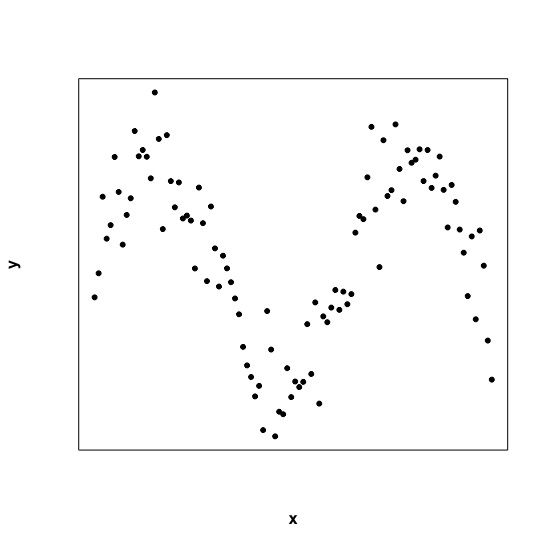
\includegraphics[width=\linewidth]{images/nonlinear_data.jpeg} 
    \end{minipage}
    \hfill
    \begin{minipage}{0.49\textwidth}
        \centering
        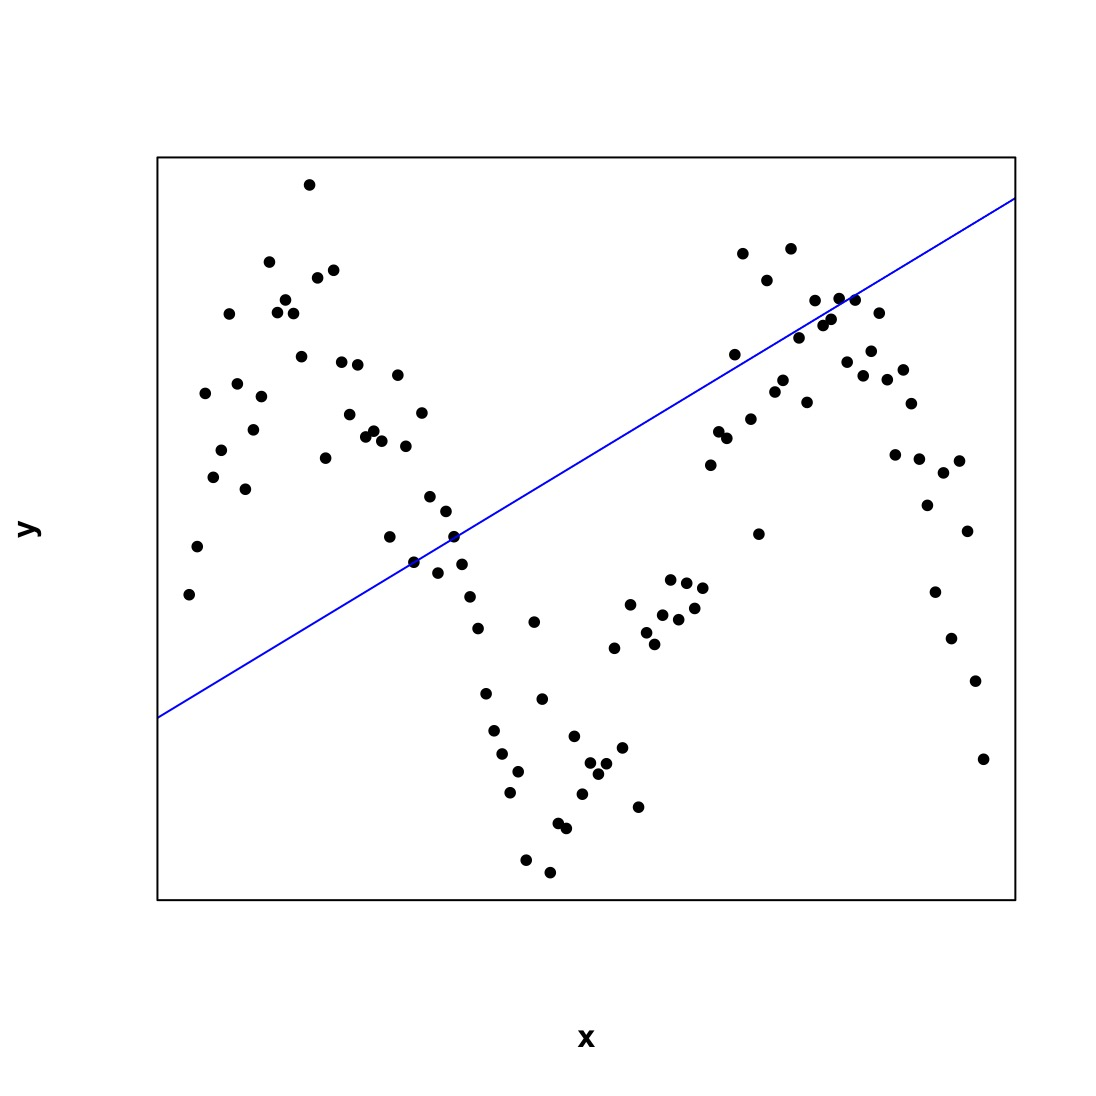
\includegraphics[width=\linewidth]{images/nonlinear_fit.jpeg} 
    \end{minipage}
    \begin{itemize}
        \item Single linear function \alertblue{under-fits} non-linear data
    \end{itemize}
\end{frame}
%------------------------------------------------
\begin{frame}{Basis function (function of predictors)}
    \begin{itemize}
        \item Known family of \alertblue{functions or transformations} e.g polynomial functions, threshold functions, regression splines etc \alertblue{applied to a predictor X to generate basis variables}: \(b_1\)(X), \(b_2\)(X),...,\(b_K\)(X).
    \begin{equation}
    \eqnmark[blue]{node1}{y}=
    \eqnmark[red]{node2}{\beta_0} +
    \eqnmark[purple]{node3}{\beta_1 b_1 (x)} + 
    \eqnmark[brown]{node4}{\beta_2 b_2 (x)} +...+
    \eqnmark[red]{node5}{\beta_k b_k (x)} +
    \eqnmark[orange]{node6}{\epsilon}
    \end{equation}
        \item For polynomial regression, the \alertblue{basis function} takes the form:
    \end{itemize}
    \begin{equation}
        \eqnmark[blue]{node1}{b_j (x)} = 
        \eqnmark[orange]{node2}{x^j} 
    \end{equation}
    \annotate[yshift=0.4em]{below, left}{node1}{polynomial function of degree j}
    \annotate[yshift=0.4em]{below, right}{node2}{Raise predictor x to degree j}

    \begin{itemize}
        \item Substituting equation (2) in (1)
    \end{itemize}
    \begin{equation*}
    \eqnmark[blue]{node1}{y}=
    \eqnmark[red]{node2}{\beta_0} +
    \eqnmarkbox[purple]{node3}{\beta_1 x} + 
    \eqnmarkbox[brown]{node4}{\beta_2 x^2} + 
    \eqnmarkbox[blue]{node5}{\beta_3 x^3} +...+
    \eqnmarkbox[red]{node6}{\beta_k x^k} +
    \eqnmark[orange]{node7}{\epsilon}
\end{equation*}
\end{frame}
%------------------------------------------------
\begin{frame}{Polynomial basis function}
    \begin{itemize}
        \item \alertblue{Extend} linear models to \alertblue{flexibly model non-linear relationships} by including polynomial terms (\(x^2\), \(x^3\),...,\(x^d\)) for a predictor
    \end{itemize}
\vspace{1.5em}  
\begin{equation*}
    \eqnmarkbox[blue]{node1}{y}=
    \eqnmarkbox[red]{node2}{\beta_0} +
    \eqnmarkbox[purple]{node3}{\beta_1 x} + 
    \eqnmarkbox[orange]{node4}{\epsilon}
\end{equation*}
\annotate[yshift=0.4em]{left}{node1}{response variable}
\annotate[yshift=-0.4em]{below,left}{node2}{intercept}
\annotate[yshift=0.4em]{above, label right}{node3}{predictor}
\annotate[yshift=-0.4em]{below, label right}{node4}{error/random term}
\vspace{0.5em}       
     \begin{itemize}
        \item Create (\alertblue{extra}) predictors by raising each of the original predictors to a power
    \end{itemize}
\vspace{1.5em}  
\begin{equation*}
    \eqnmark[blue]{node1}{y_i}=
    \eqnmark[red]{node2}{\beta_0} +
    \eqnmarkbox[purple]{node3}{\beta_1 x} + 
    \eqnmarkbox[brown]{node4}{\beta_2 x^2} + 
    \eqnmarkbox[blue]{node5}{\beta_3 x^3} +...+
    \eqnmarkbox[red]{node6}{\beta_d x^d} +
    \eqnmark[orange]{node7}{\epsilon}
\end{equation*}
\annotate[yshift=0.4em]{above, left}{node3}{Linear term (degree 1)}
\annotate[yshift=-0.4em]{below, left}{node4}{Degree 2 polynomial}
\annotate[yshift=-0.4em]{below, right}{node5}{Degree 3 polynomial}
\annotate[yshift=0.4em]{above, left}{node6}{Degree d polynomial}
\vspace{1em}  
\end{frame}
%------------------------------------------------
\begin{frame}{Polynomial regression}
    \begin{itemize}
        \item \alertblue{Unknown coefficients $\beta_1$, $\beta_2$...$\beta_d$} can be easily estimated using least squares because this is just a \alertblue{linear model with non-linear function of predictors} (\(x\), \(x^2\), \(x^3\),...,\(x^d\))
        \item Unusual to use \(d\) greater than \alertblue{3 or 4}, \alert{overfitting and wiggly} 
    \end{itemize}
    \centering
    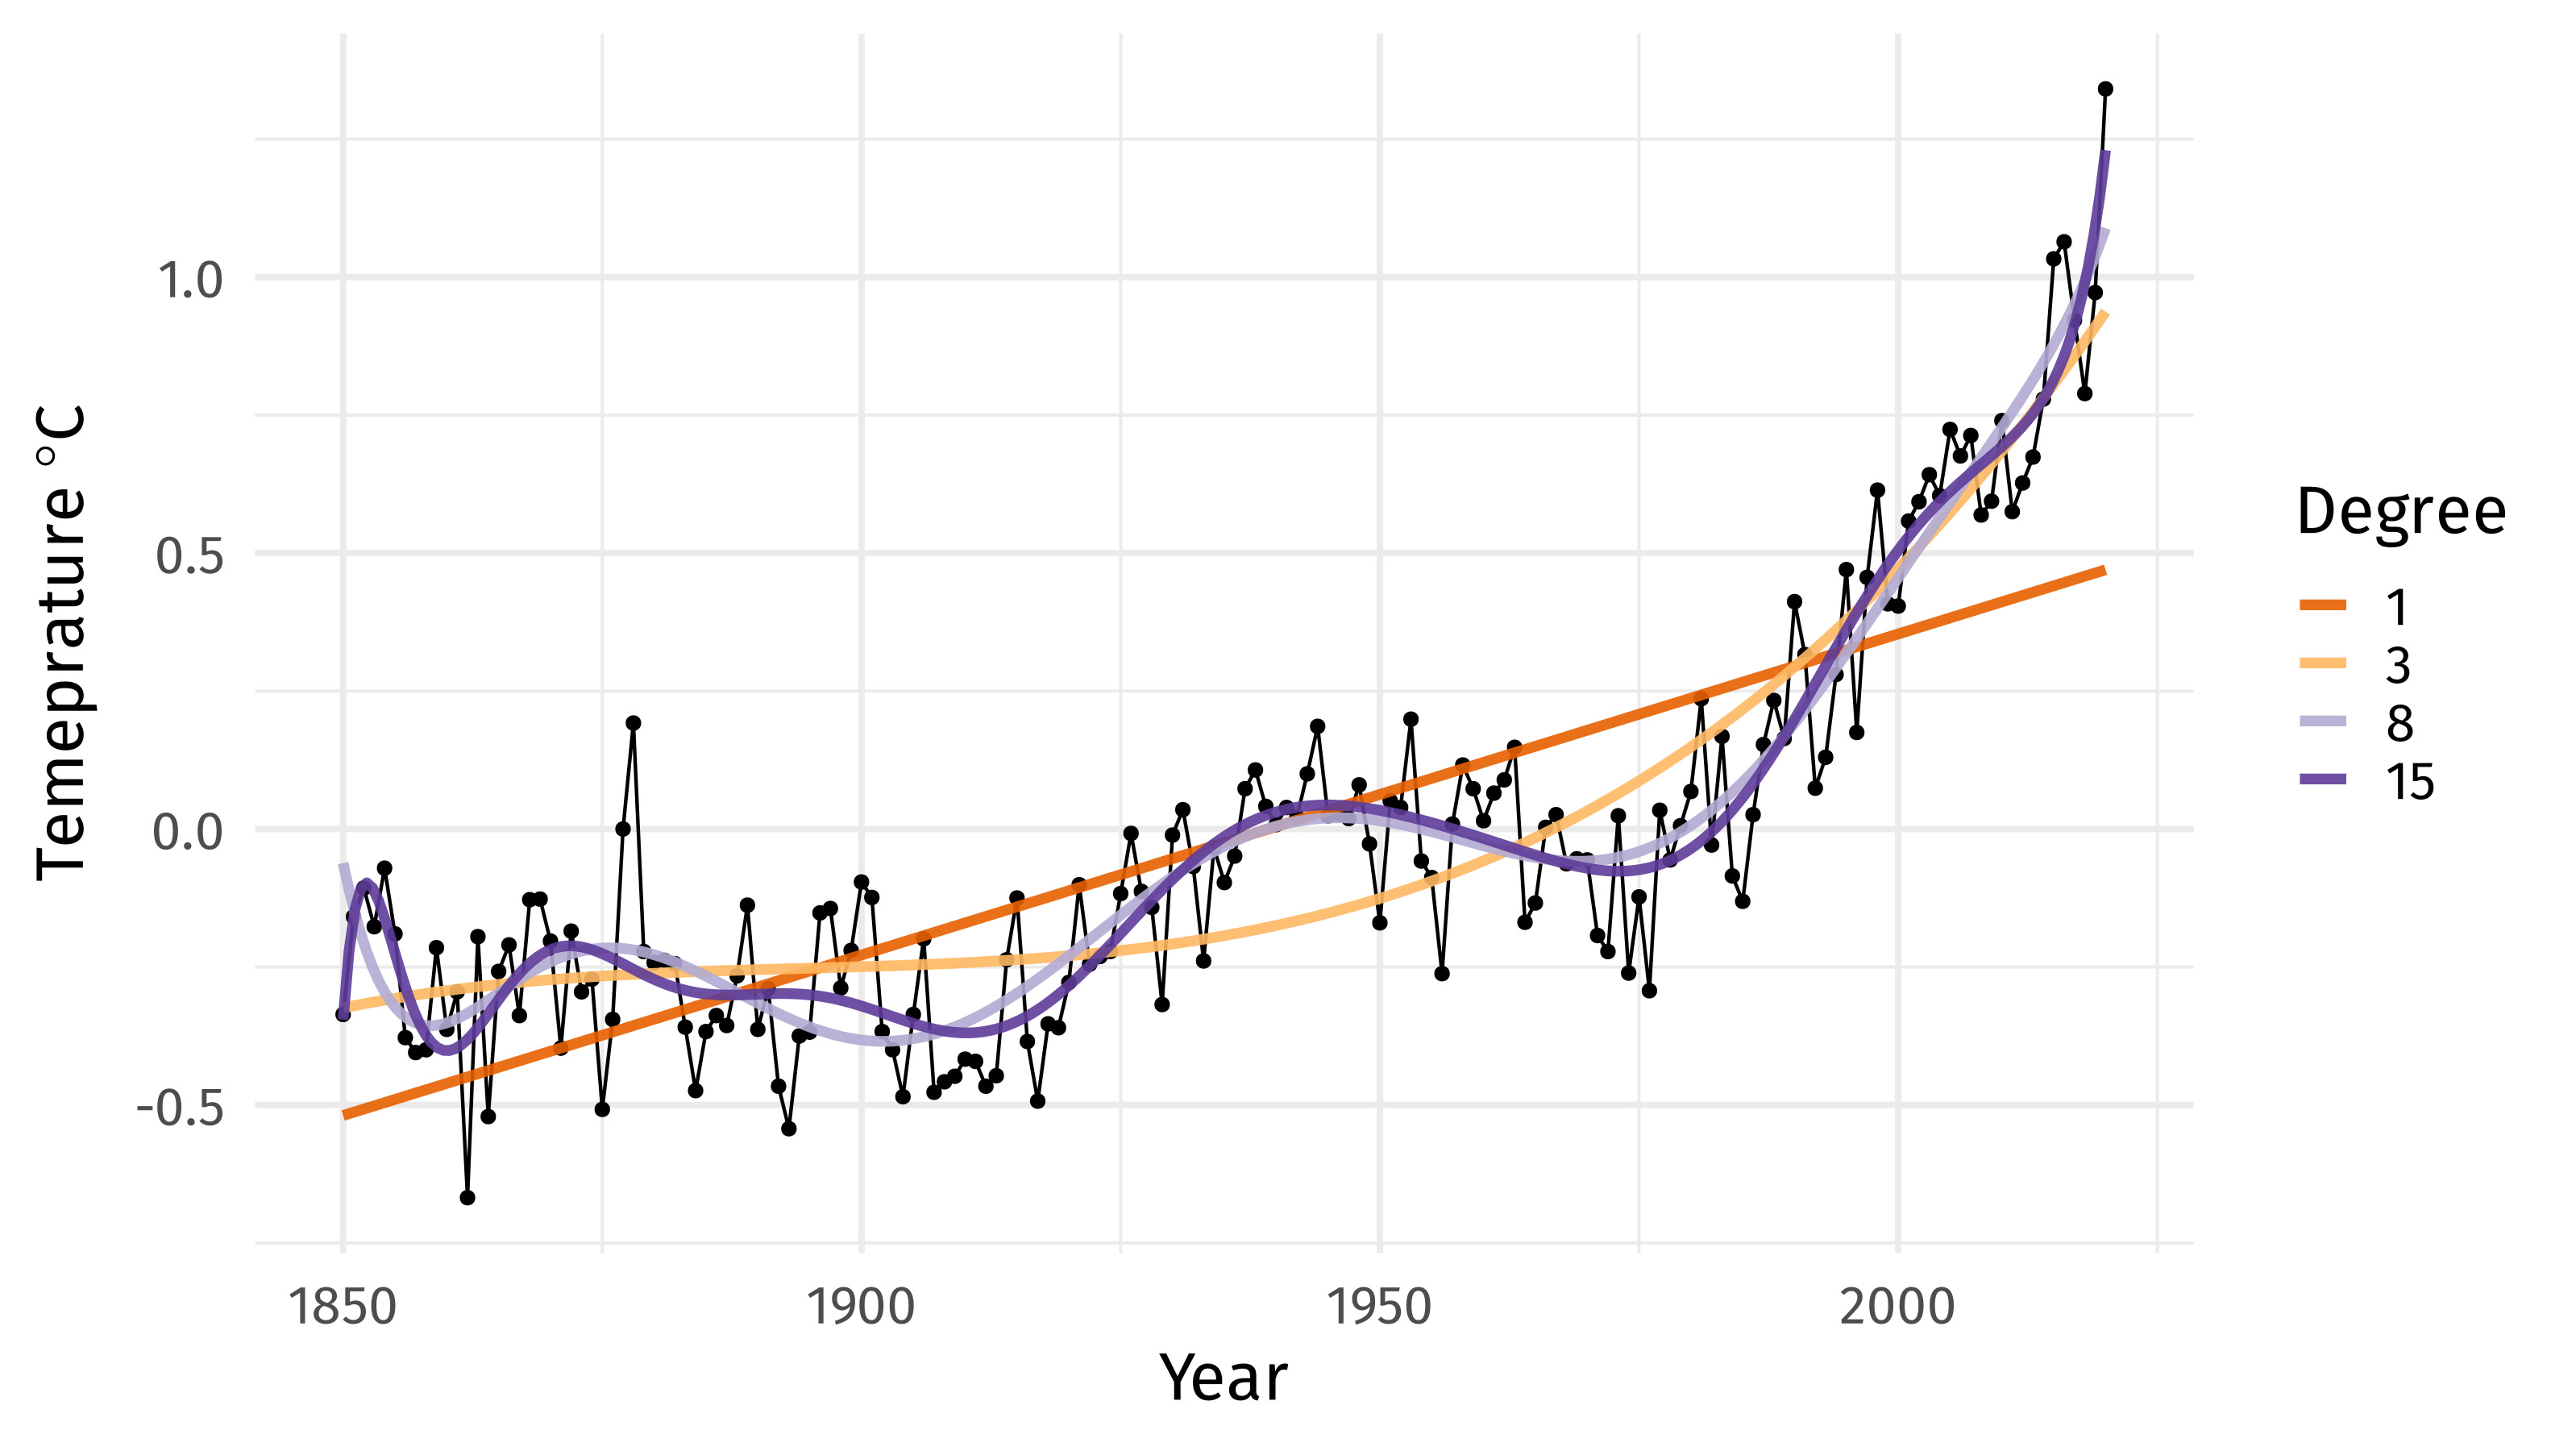
\includegraphics[width=8cm,keepaspectratio]{images/overfit.jpg}
\end{frame}
%------------------------------------------------
\section{Piecewise Polynomials}
\begin{frame}{Modelling non-linear relationships: knots}
    \begin{columns}
        \begin{column}{0.65\textwidth}
            \begin{itemize}
                \item A first step is to "divide" the predictor into sections and generate individual regressions in each  
                \item These divisions happen at positions called \alertblue{knots, \(\xi\)} 
                \item \alertblue{Coefficients} change at knots, more knots in places where we feel the \alertblue{function might vary most rapidly}
            \end{itemize}
        \end{column}
        \begin{column}{0.49\textwidth}
            \centering
            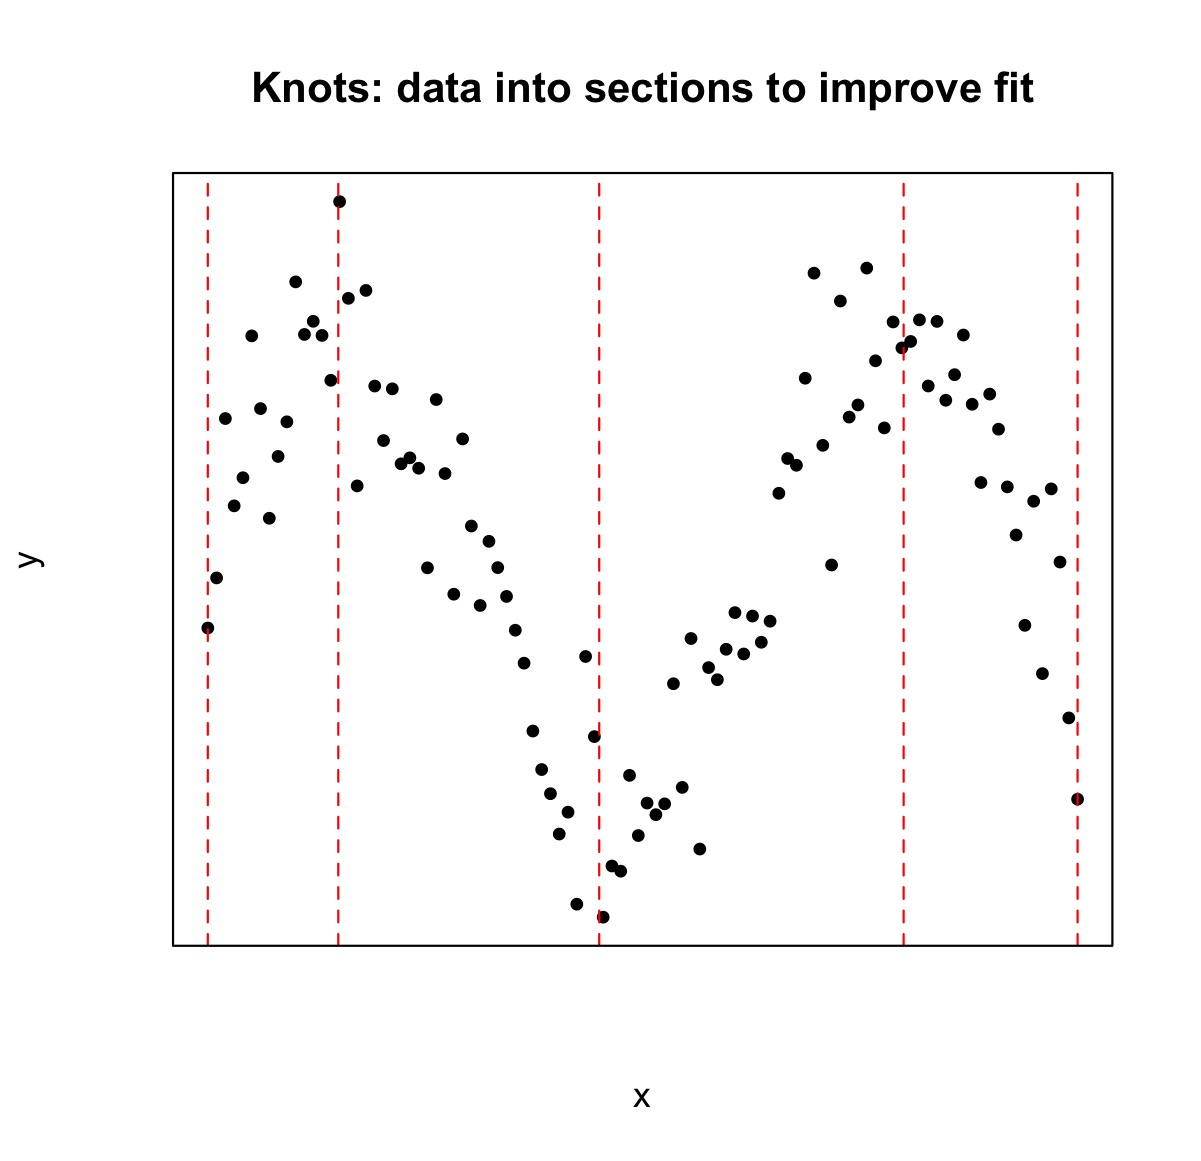
\includegraphics[width=\linewidth]{images/knots.jpeg} 
        \end{column}
    \end{columns}
\end{frame}
%------------------------------------------------
\begin{frame}{Piecewise polynomial regression}
     \centering
     \begin{columns}
         \begin{column}{0.55\textwidth}
     {\scriptsize
          \begin{equation*}
             \eqnmark[blue]{node1}{y_i}=
               \begin{cases} 
                  \eqnmark[red]{node2}{\beta_0{}_1} + 
                  \eqnmark[purple]{node3}{\beta_{11}x} + 
                  \eqnmark[orange]{node4}{\epsilon} & \text{if } 
                  \eqnmark{node5}{x < \xi_1,} \\
                  \eqnmark[red]{node2}{\beta_0{}_2} + 
                  \eqnmark[purple]{node3}{\beta_{12}x} + 
                  \eqnmark[orange]{node4}{\epsilon} & \text{if } 
                  \eqnmark{node5}{\xi_1 \geq x < \xi_2,} \\
                  \eqnmark[red]{node2}{\beta_0{}_3} + 
                  \eqnmark[purple]{node3}{\beta_{13}x} + 
                  \eqnmark[orange]{node4}{\epsilon} & \text{if } 
                  \eqnmark{node5}{\xi_2\geq x < \xi_3,} \\
                  \eqnmark[red]{node2}{\beta_0{}_4} + 
                  \eqnmark[purple]{node3}{\beta_{14}x} + 
                  \eqnmark[orange]{node4}{\epsilon} & \text{if } 
                  \eqnmark{node5}{\xi_3 \geq x < \xi_4.} 
              \end{cases}
          \end{equation*}
          }
          \end{column}
          \begin{column}{0.5\textwidth}
             \centering
            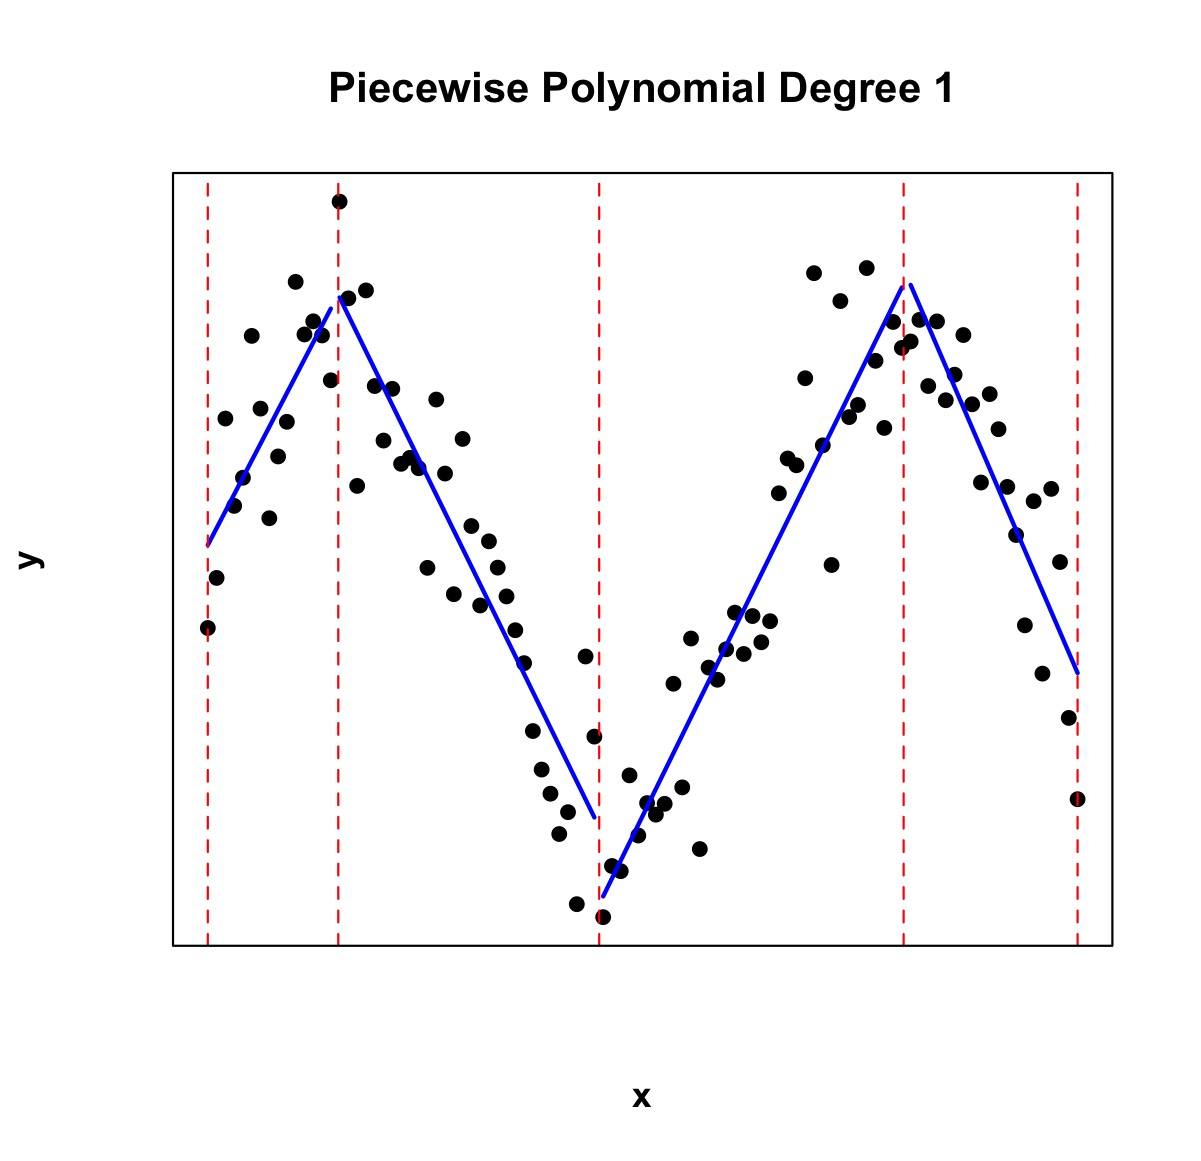
\includegraphics[width=\linewidth, height=0.6\textheight, keepaspectratio]{images/piecewise_degree_1.jpeg}  
          \end{column}      
    \end{columns}
    \begin{itemize}
        \item Applying \alertblue{degree 1 polynomial basis functions} to predictor \\ X to generate \alertblue{basis variables of X, "piecewise"}
    \end{itemize}
\end{frame}
%------------------------------------------------
\begin{frame}{Piecewise polynomial regression}
    
    \begin{columns}
        \begin{column}{0.47\textwidth}
            \centering
            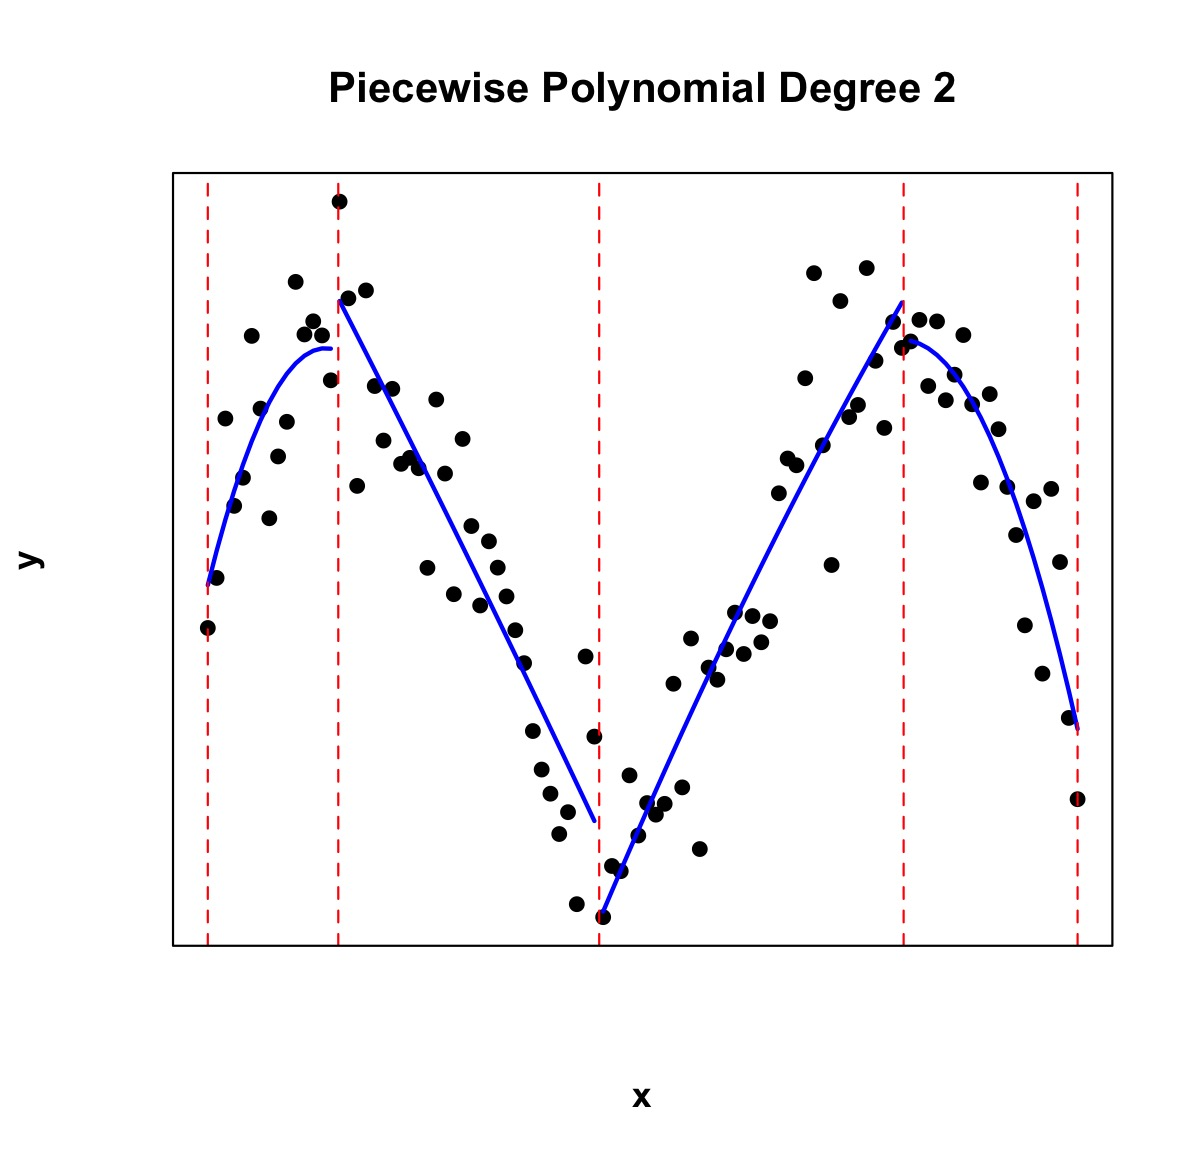
\includegraphics[width=\linewidth]{images/piecewise_degree_2.jpeg} 
        \end{column}
        \begin{column}{0.47\textwidth}
            \centering
            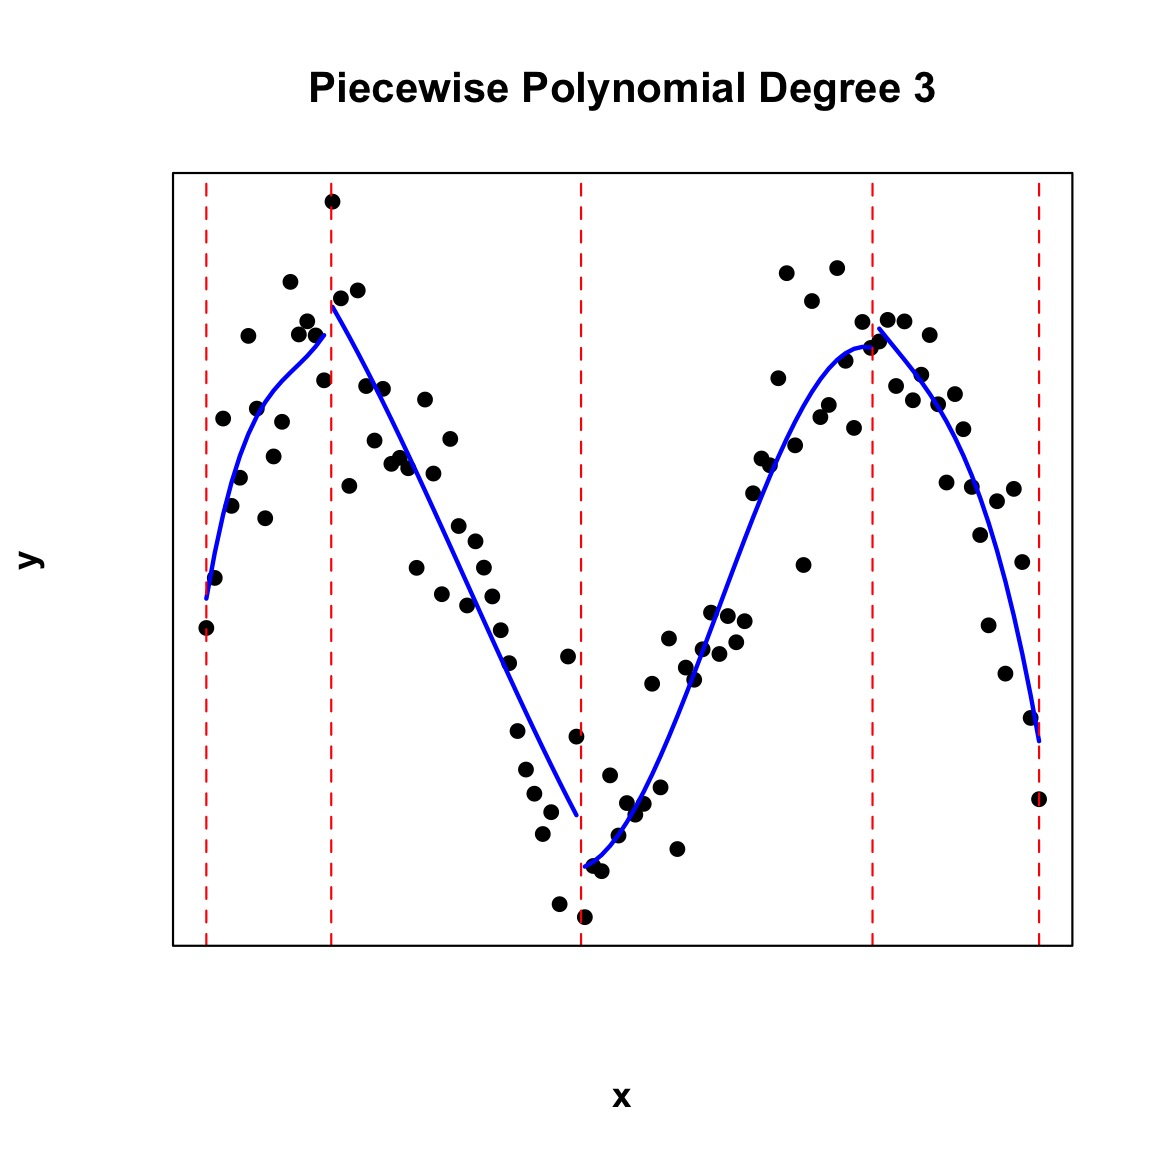
\includegraphics[width=\linewidth]{images/piecewise_degree_3.jpeg} 
        \end{column}
    \end{columns}  
    \begin{itemize}
        \item A major pathology to notice in all of the above examples is the \alertblue{discontinuity} at the knots (\alertblue{unconstrained polynomials}) 
        \item Unconstrained here means \alertblue{no restrictions of continuity imposed} at knots
    \end{itemize}
\end{frame}
%------------------------------------------------
\section{Regression Splines}
\begin{frame}{Regression Splines}
    \begin{itemize}
        \item We want \alertblue{continuity} at the knots, and \alertblue{smoothness} of the overall curve, we \alertblue{impose continuity constraints} 
        \item \alertblue{Regression spline} with knots at \alertblue{$\xi_k$, k=1,...,K} is a piecewise polynomial \alertblue{continuous at each knot}
        \item  \alertblue{Linear spline} is represented with a basis for a linear polynomial x and one \alertblue{truncated power basis function} per knot
        \vspace{0.5cm}
    \end{itemize}    
    \begin{equation*}
        \eqnmark[blue]{node1}{y} =
        \eqnmark[red]{node2}{\beta_0} +
        \eqnmarkbox[purple]{node3}{\beta_1 x} +
        \sum_{k=1}^{K} \eqnmarkbox[brown]{node4}{\beta_k (x - \xi_k)_+} +
        \eqnmark[orange]{node5}{\epsilon}
    \end{equation*}
    \annotate[yshift=1.2em]{above, right}{node3}{Linear polynomial term (degree 1)}
    \annotate[yshift=-0.8em]{below, right}{node4}{Truncated power basis}
    \begin{itemize}
        \item Ensures \alertblue{continuity} at knots
    \end{itemize}
\end{frame}
%------------------------------------------------
\begin{frame}{Truncated power basis function}
 \begin{columns}
     \begin{column}{0.6\textwidth} 
         \centering
         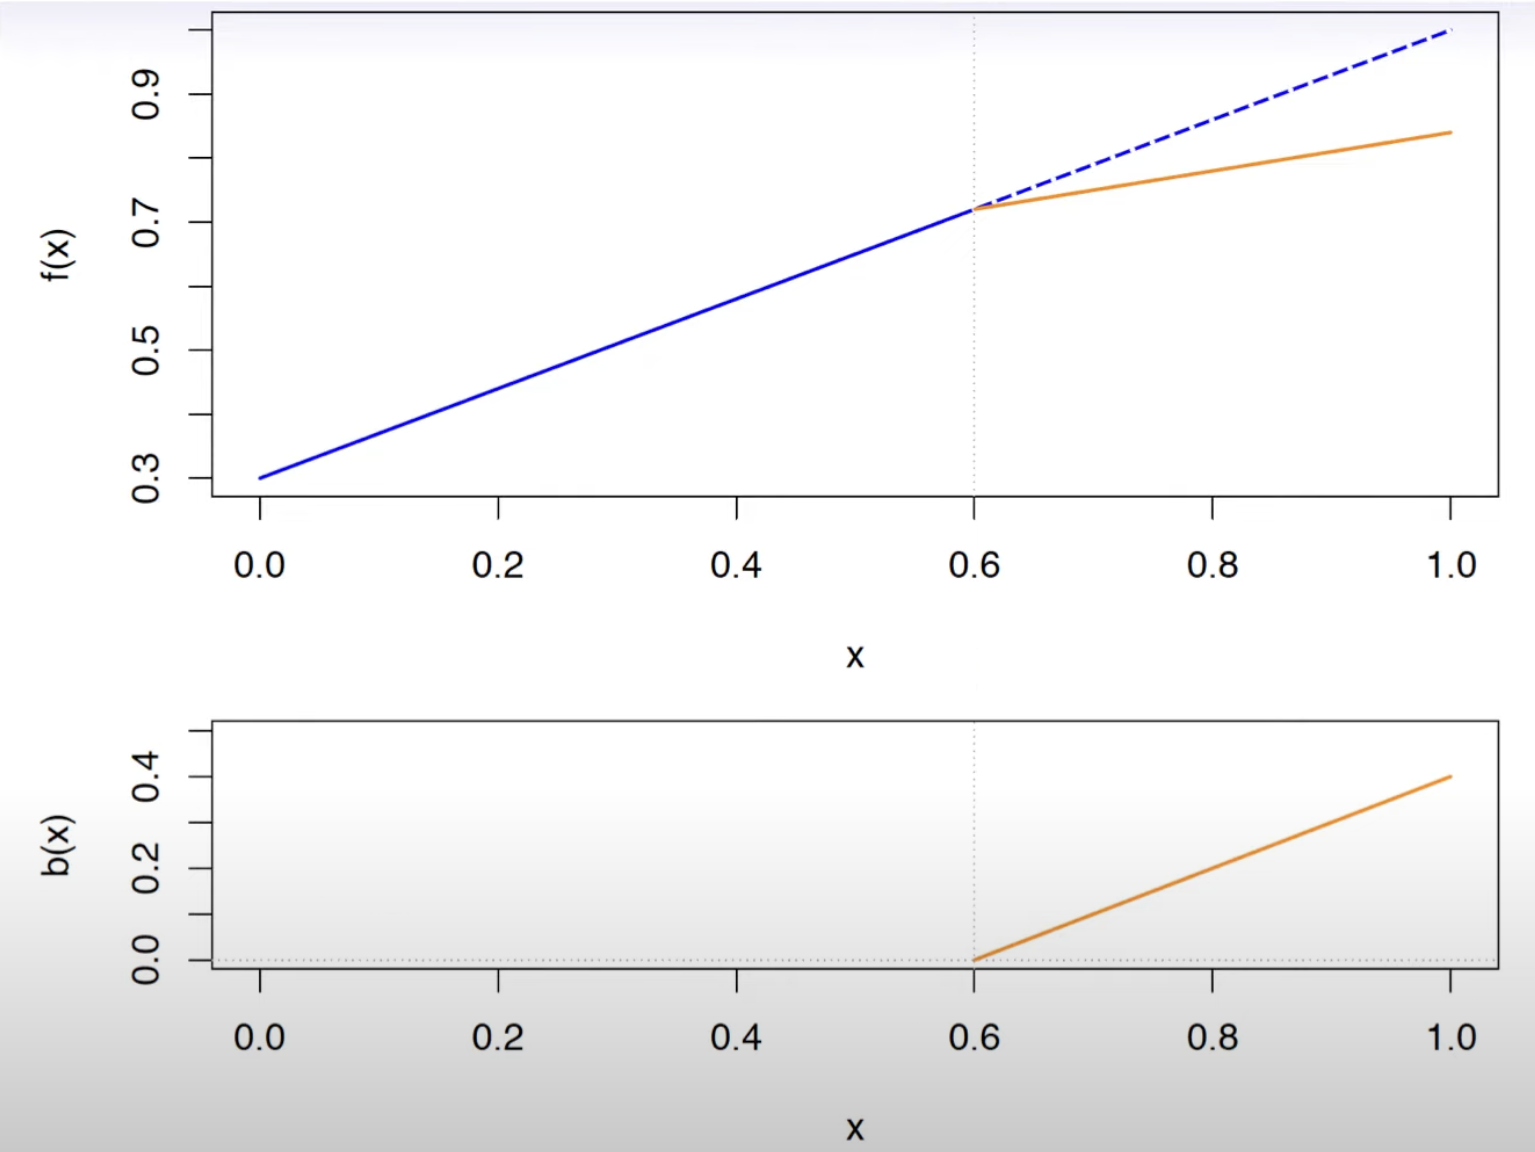
\includegraphics[width=6.5cm,keepaspectratio]{images/truncated_linear.png}
     \end{column}
     \begin{column}{0.5\textwidth} 
         \begin{itemize}
             \item Truncated power basis function is \alertblue{zero} for \alertblue{\( x < \xi_k \)} and \alertblue{nonzero} only for \alertblue{\( x \geq \xi_k \)}
         \end{itemize}
         \begin{equation*}
             \alertblue{(x - \xi)_+} =
             \begin{cases}
                 \alertblue{(x - \xi)}, & \text{if } x \geq \xi \\
                 \textcolor{red}{0}, & \text{otherwise}
             \end{cases}
         \end{equation*}
         \begin{itemize}
             \item Linear spline representation using truncated power basis function at \alertblue{knot, \(\xi\) = 0.6}
         \end{itemize}
     \end{column}
 \end{columns}
\end{frame}
%------------------------------------------------
% \begin{frame}{Truncated Power Basis Function}
%  \begin{columns}
%      \begin{column}{0.6\textwidth} 
%          \centering
%          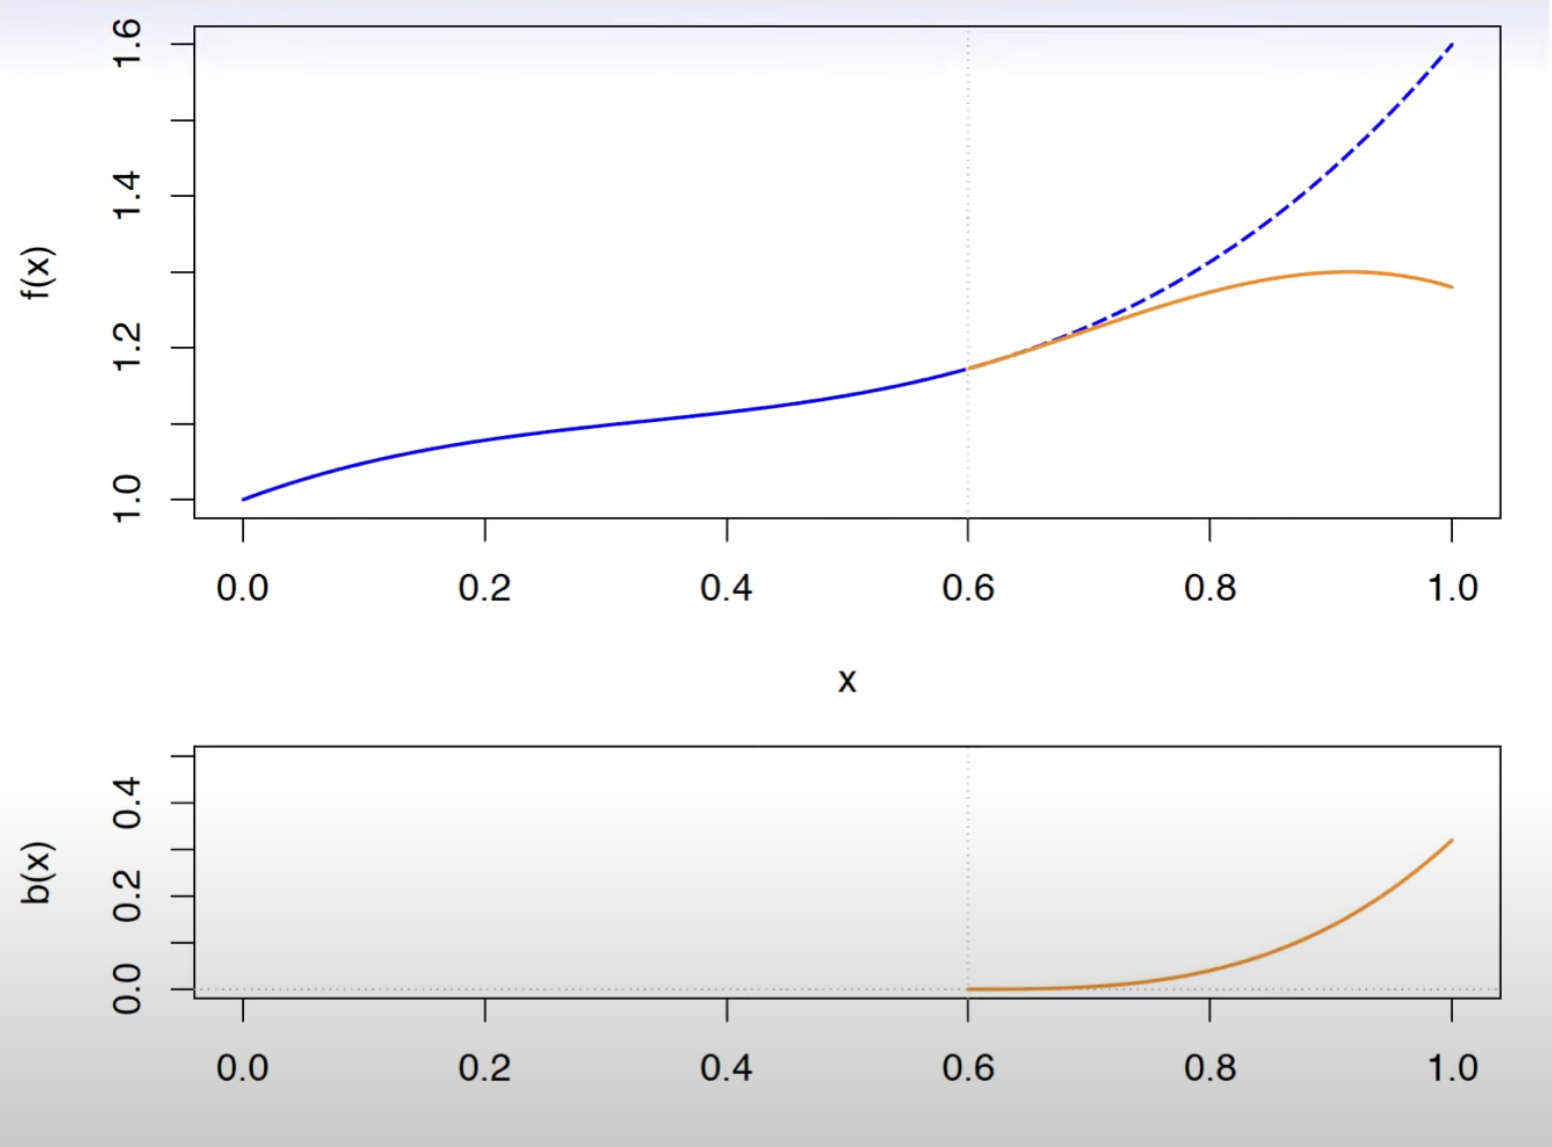
\includegraphics[width=6.5cm,keepaspectratio]{images/truncated_cubic.png}
%      \end{column}
%      \begin{column}{0.5\textwidth} 
%          \begin{itemize}
%              \item Truncated power basis function is \alertblue{zero} for \alertblue{\( x < \xi_k \)} and \alertblue{nonzero} only for \alertblue{\( x \geq \xi_k \)}
%          \end{itemize}
%          \begin{equation*}
%              \alertblue{(x - \xi)^3_+} =
%              \begin{cases}
%                  \alertblue{(x - \xi)^3}, & \text{if } x \geq \xi \\
%                  \textcolor{red}{0}, & \text{otherwise}
%              \end{cases}
%          \end{equation*}
%          \begin{itemize}
%              \item Cubic spline representation using truncated power basis function at \alertblue{knot, \(\xi\) = 0.6}
%          \end{itemize}
%      \end{column}

%  \end{columns}
% \end{frame}
% %------------------------------------------------
\begin{frame}{Linear spline}%{$C^0$ Continuity}
    % \begin{itemize}
    %     \item \alertblue{Function values} must match at each knot, $\xi$, meaning there are \alertblue{no gaps or jumps} e.g for a \alertblue{linear spline}
    % \end{itemize}
        \begin{equation*}
            \eqnmark[blue]{node1}{y} =
            \eqnmark[red]{node2}{\beta_0} +
            \eqnmarkbox[purple]{node3}{\beta_1 x} +
            \eqnmarkbox[brown]{node4}{\beta_2 (x - \xi)_+} +
            \eqnmark[orange]{node5}{\epsilon}
        \end{equation*}
        \annotate[yshift=0.5em]{above, left}{node4}{Ensures continuity at knots}

    \begin{columns}
        \begin{column}{0.45\textwidth}
            \centering
            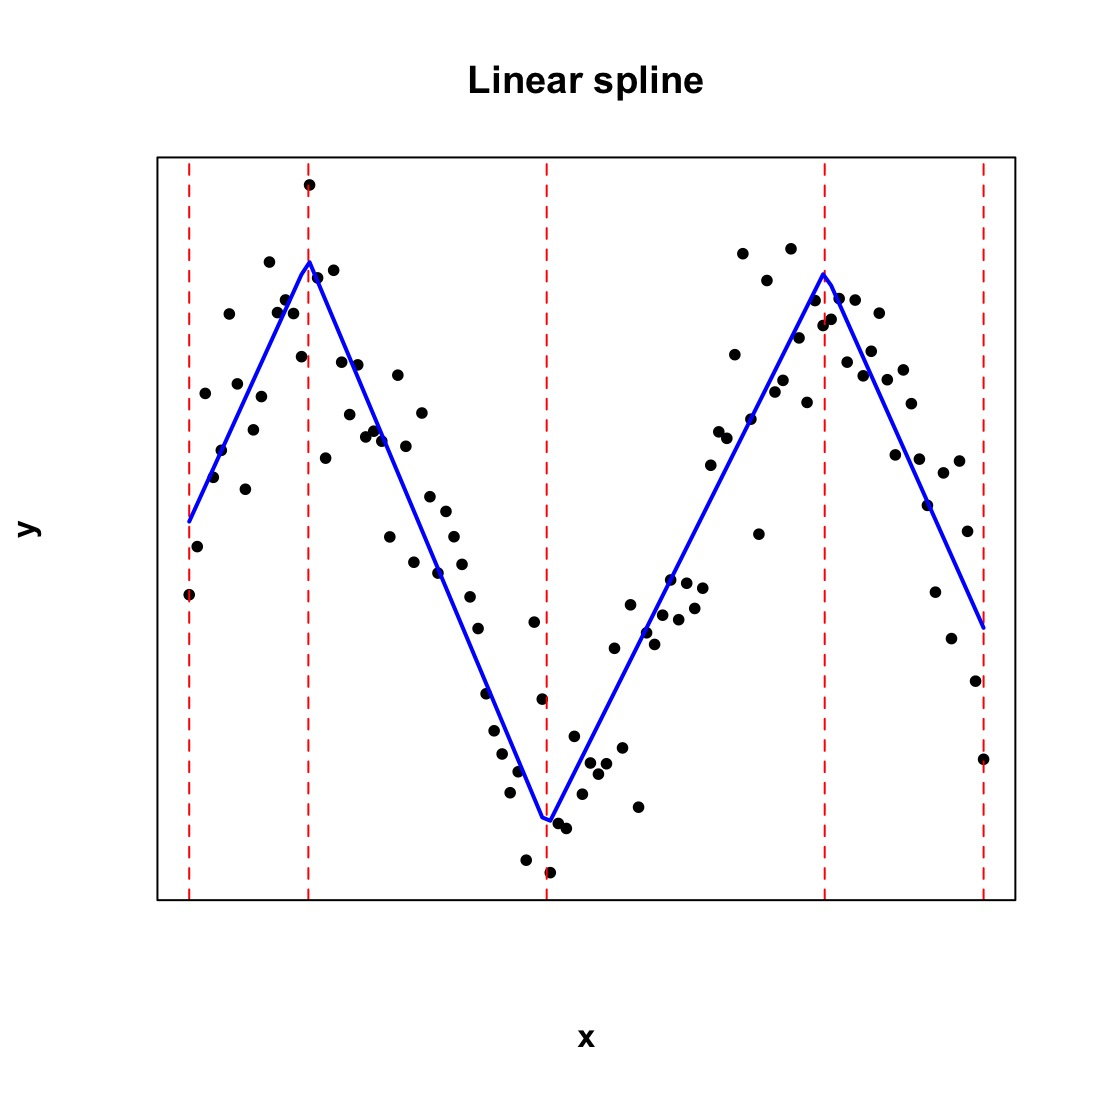
\includegraphics[width=\linewidth]{images/linear_spline.jpeg} 
        \end{column}
        \begin{column}{0.7\textwidth}
            {\scriptsize
             \begin{equation*}
             \eqnmark[blue]{node1}{y}=
               \begin{cases} 
                  \eqnmark[red]{node2}{\beta_0} + 
                  \eqnmark[purple]{node3}{\beta_1 x} + 
                  \eqnmark[orange]{node4}{\epsilon} & \text{if } 
                  \eqnmark{node5}{x < \xi_1,} \\
                  \eqnmark[red]{node2}{..} + 
                  \eqnmark[blue]{node3}{\beta_2 (x - \xi_1) } +
                  \eqnmark[orange]{node4}{\epsilon} & \text{if } 
                  \eqnmark{node5}{\xi_1 \geq x < \xi_2,} \\
                  \eqnmark[red]{node2}{...} + 
                  \eqnmark[blue]{node3}{\beta_3 (x - \xi_2)} +
                  \eqnmark[orange]{node4}{\epsilon} & \text{if } 
                  \eqnmark{node5}{\xi_2\geq x < \xi_3,} \\
                  \eqnmark[red]{node2}{....} + 
                  \eqnmark[blue]{node3}{\beta_4 (x - \xi_3)} +
                  \eqnmark[orange]{node4}{\epsilon} & \text{if } 
                  \eqnmark{node5}{\xi_3 \geq x < \xi_4.} 
              \end{cases}
          \end{equation*}
          }
        \end{column}
    \end{columns}
    \begin{itemize}
        \item \alertblue{\( \xi_1 \geq x < \xi_2 \)}, first truncated basis \alertblue{activated}, \alert{adding a slope change} 
    \end{itemize} 
\end{frame}
%------------------------------------------------
\begin{frame}{Quadratic vs cubic spline}
\begin{columns}
    \begin{column}{0.5\textwidth}
        \centering
        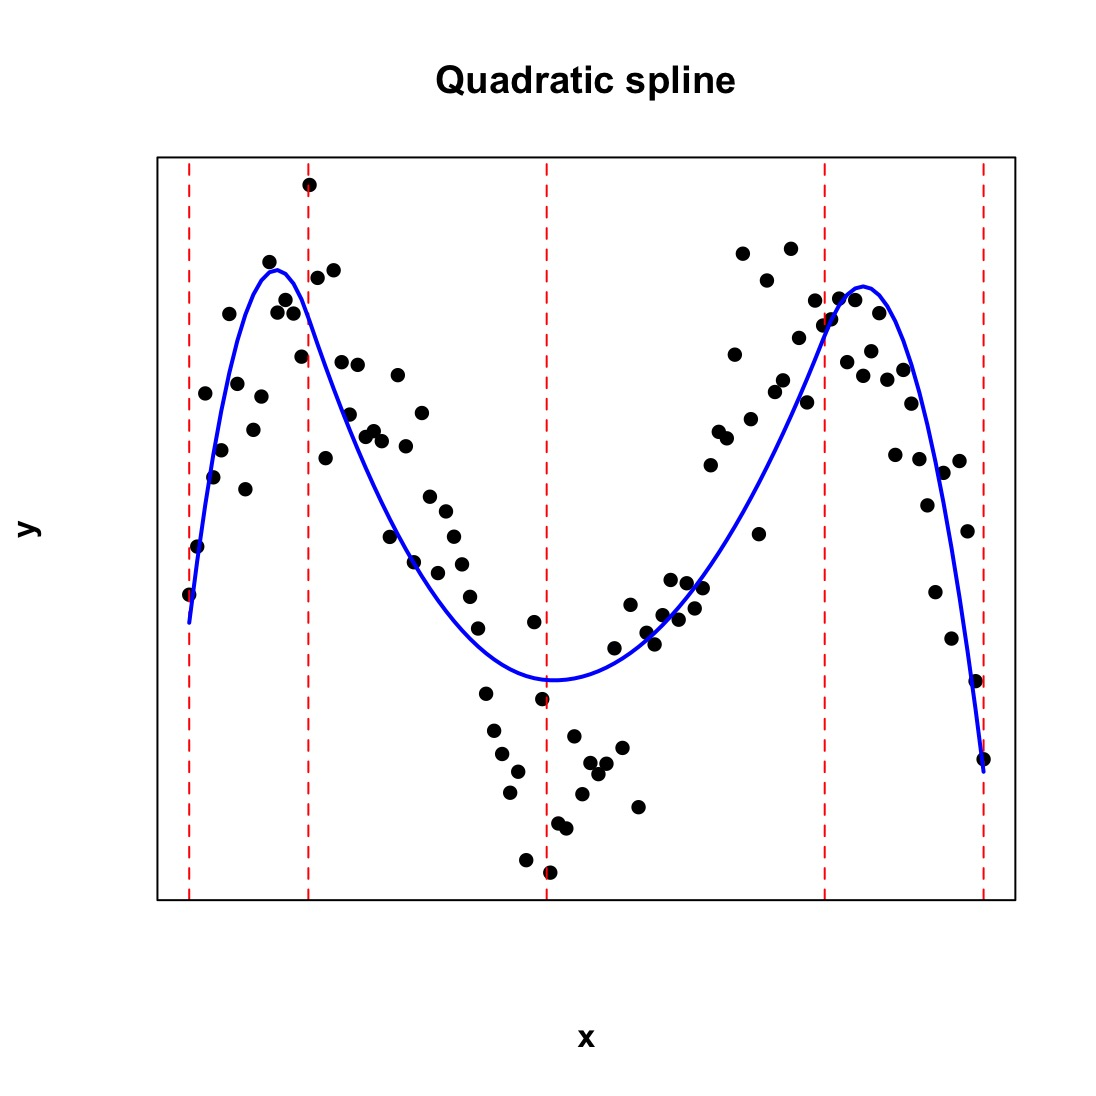
\includegraphics[width=\linewidth]{images/quadratic_spline.jpeg} 
    \end{column}
    \begin{column}{0.5\textwidth}
        \centering
        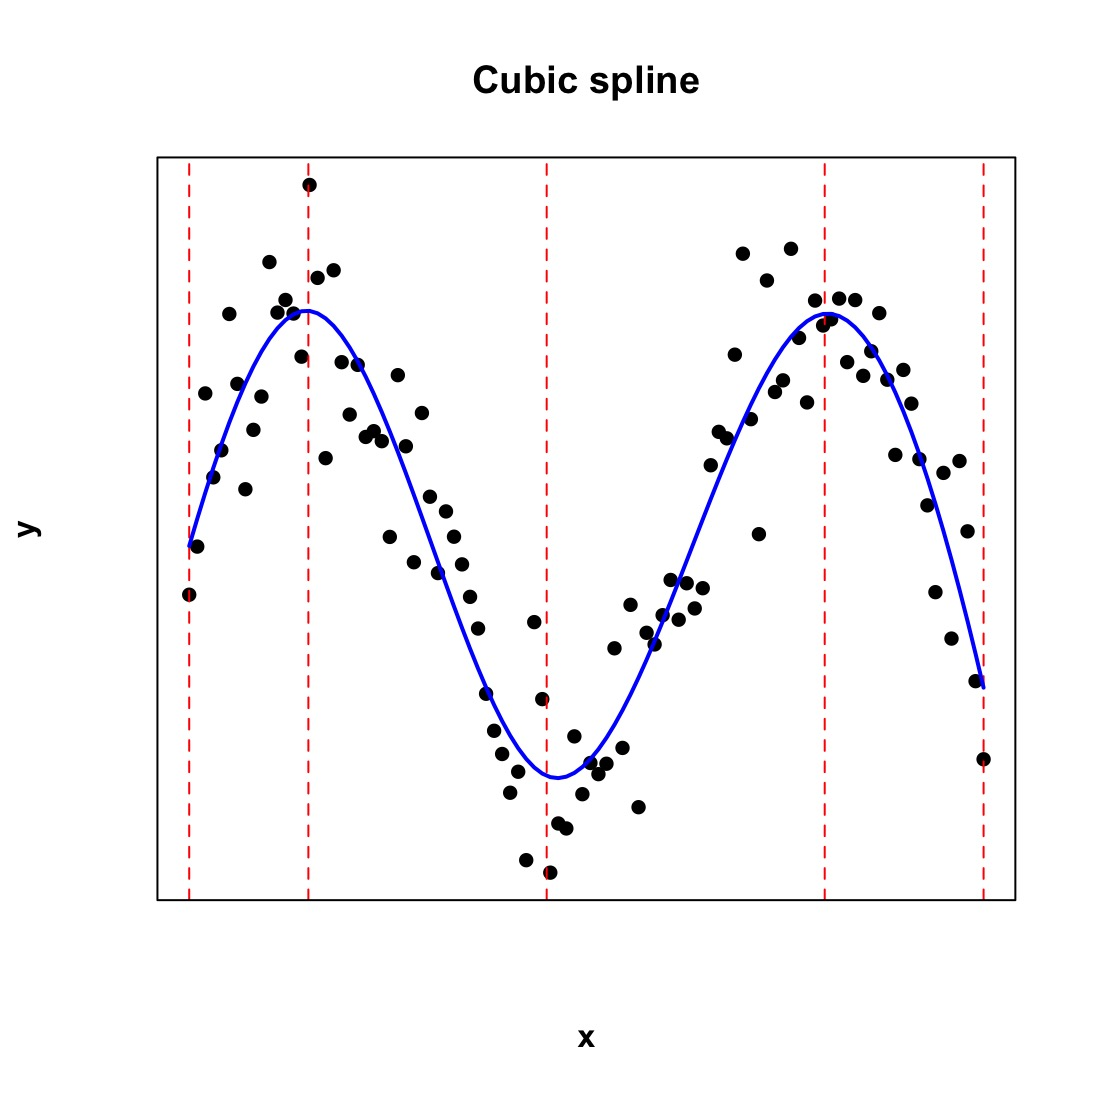
\includegraphics[width=\linewidth]{images/cubic_spline.jpeg} 
    \end{column}
\end{columns}
    \begin{itemize}
        \item The \alertblue{cubic spline} has a \alertblue{more smooth curvature} and \alertblue{fits the data better} than the \alertblue{quadratic spline}  
    \end{itemize}
\end{frame}
%------------------------------------------------
% \begin{frame}{$C^1$ Continuity}
%      \begin{itemize}
%          \item \alertblue{First derivative} must be continuous at each knot, $\xi$, ensuring \alertblue{no abrupt changes in curvature/direction i.e no sharp ends} e.g for a \alertblue{quadratic spline}
%      \end{itemize}    
%     \begin{columns}
%         \begin{column}{0.5\textwidth}
%             \centering
%             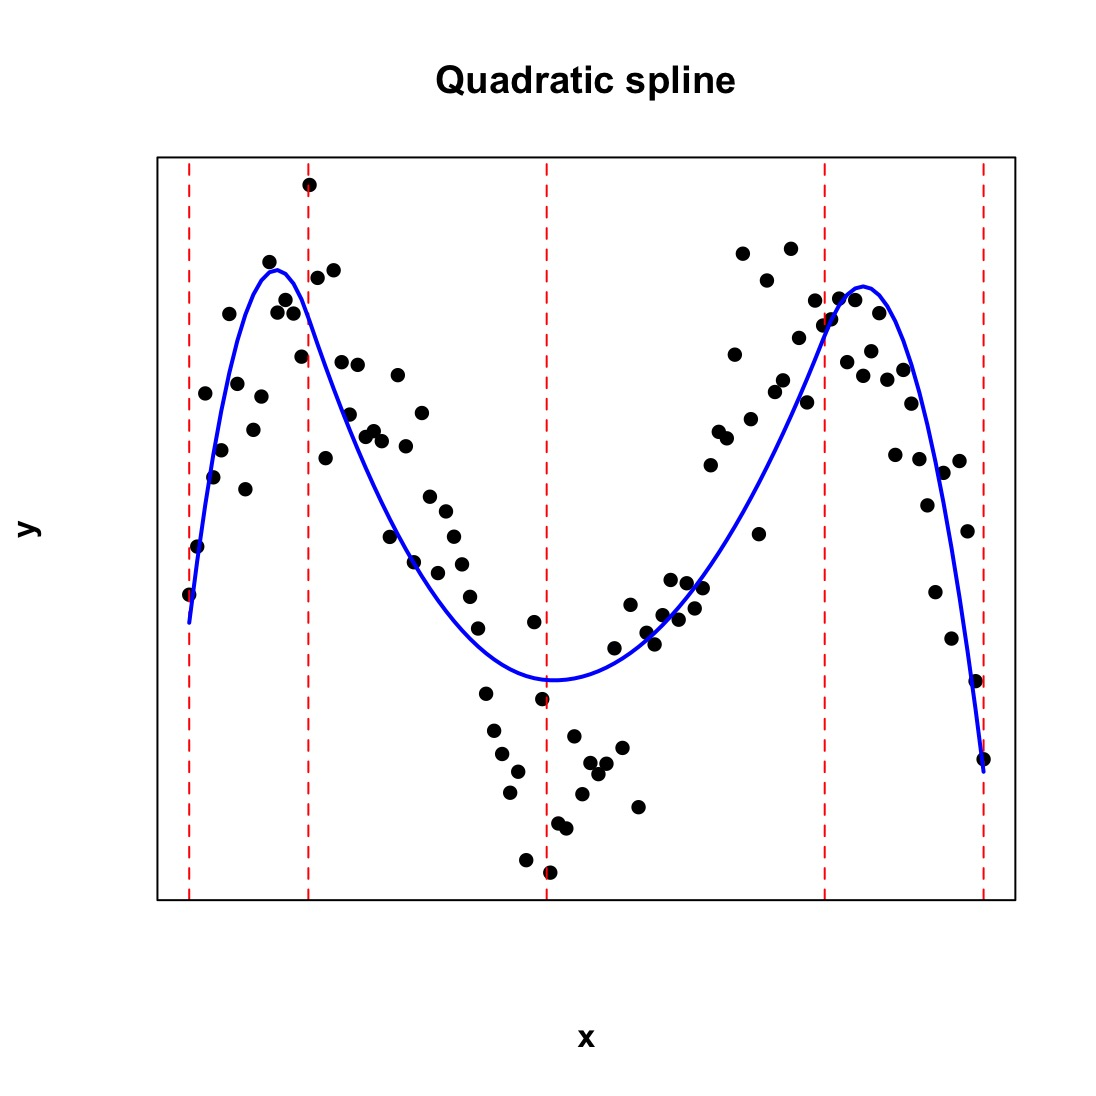
\includegraphics[width=\linewidth]{images/quadratic_spline.jpeg} 
%         \end{column}
%         \begin{column}{0.65\textwidth}
%             \begin{equation*}
%            \alertblue{(x - \xi)^2_+} = 
%            \begin{cases} 
%            \alertblue{(x - \xi)^2}, & x > \xi \\ 
%            0, & x \leq \xi 
%            \end{cases}
%         \end{equation*}
        
%         \begin{equation*}
%          \alertblue{\frac{d}{dx}(x - \xi)^2_+} = 
%          \begin{cases} 
%          \alertblue{2(x - \xi)}, & x > \xi \\ 
%          0, & x \leq \xi 
%          \end{cases}
%        \end{equation*} 
%         \end{column}
%     \end{columns}
% \end{frame}
% %------------------------------------------------
% \begin{frame}{$C^2$ Continuity}
%     \begin{itemize}
%         \item \alertblue{Second derivative} must be continuous at each knot, $\xi$, ensuring \alertblue{ smooth curvature} e.g for a \alertblue{cubic spline}
%     \end{itemize}        
%     \begin{columns}
%     \begin{column}{0.5\textwidth}
%             \centering
%             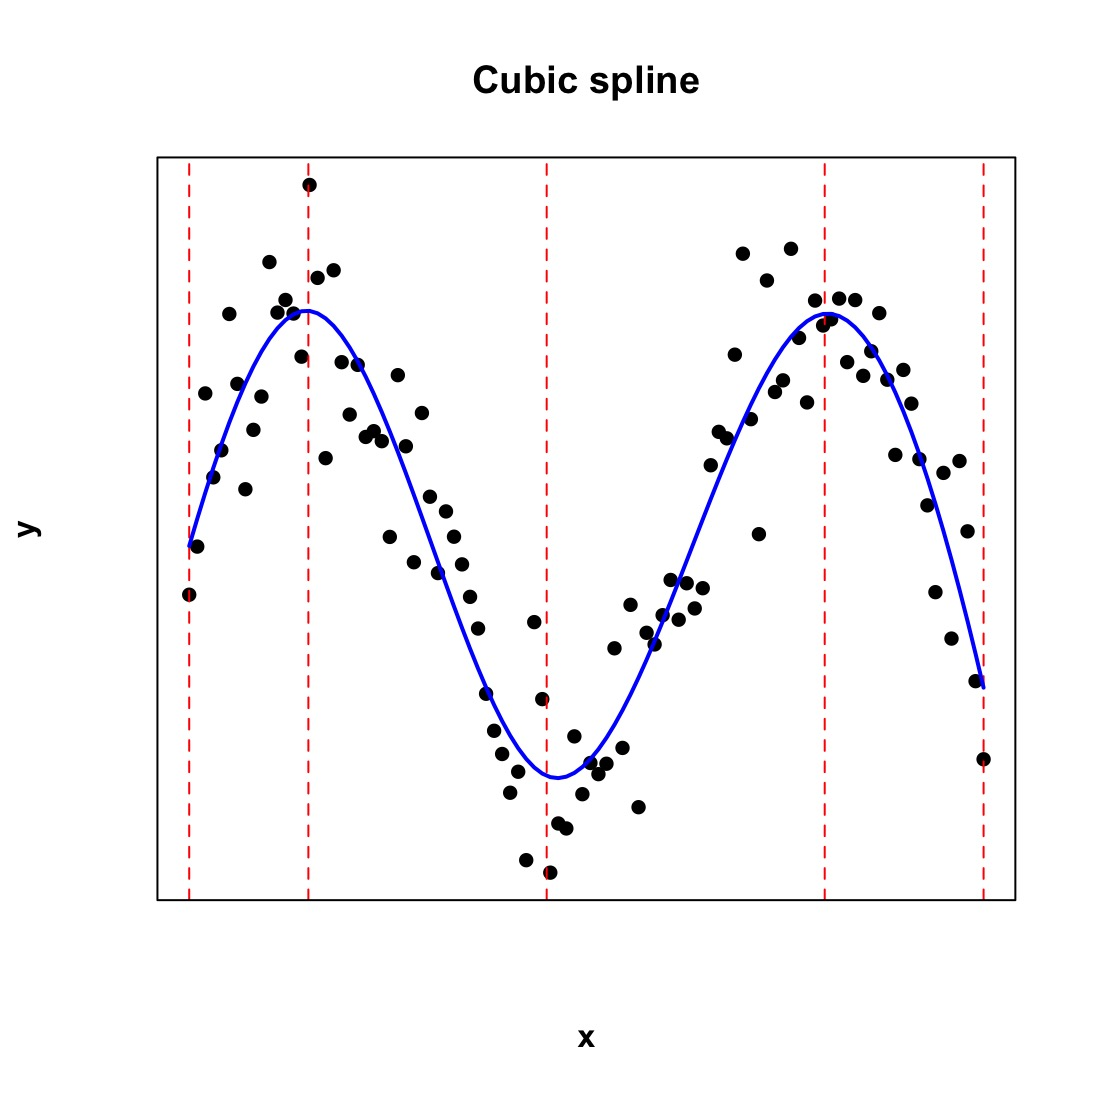
\includegraphics[width=\linewidth]{images/cubic_spline.jpeg} 
%         \end{column}
%         \begin{column}{0.7\textwidth}
%         \begin{equation*}
%            \alertblue{(x - \xi)^3_+} = 
%            \begin{cases} 
%            \alertblue{(x - \xi)^3}, & x > \xi \\ 
%            0, & x \leq \xi 
%            \end{cases}
%         \end{equation*}
        
%         \begin{equation*}
%          \alertblue{\frac{d}{dx}(x - \xi)^3_+} = 
%          \begin{cases} 
%          \alertblue{3(x - \xi)^2}, & x > \xi \\ 
%          0, & x \leq \xi 
%          \end{cases}
%        \end{equation*}

%        \begin{equation*}
%          \alertblue{\frac{d^2}{dx^2}(x - \xi)^3_+} = 
%          \begin{cases} 
%          \alertblue{6(x - \xi)}, & x > \xi \\ 
%          0, & x \leq \xi 
%          \end{cases}
%        \end{equation*}
%       \end{column}
%         \end{columns}
%     \begin{itemize}   
%         \item The cubic spline has a \alertblue{more smooth curvature} and \alertblue{fits the data better} than the quadratic spline 
%     \end{itemize}    
% \end{frame}
% %------------------------------------------------
% \begin{frame}{Comparison of Splines}
%     \centering
%     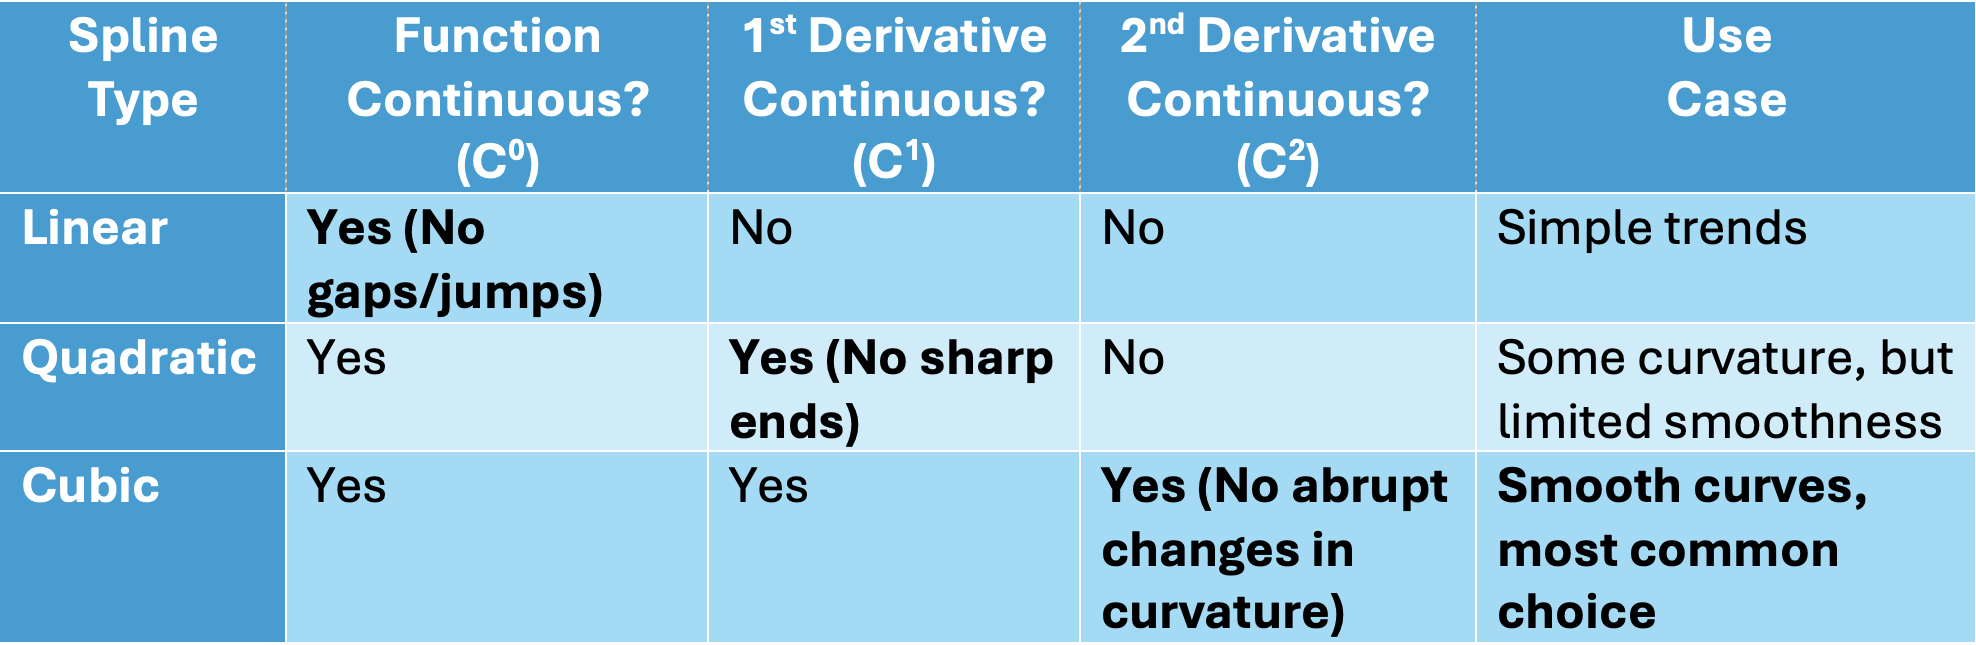
\includegraphics[width=11cm,keepaspectratio]{images/comparison_splines.png}
%     \begin{itemize}
%         \item Cubic splines, seem to be the best tool we have so far, right? \alertblue{Well, there is always room for improvement}
%     \end{itemize}
% \end{frame}
%------------------------------------------------
\begin{frame}{Limitation of these splines}
    \begin{itemize}
        \item Cubic splines, seem to be the best tool we have so far, right? \alertblue{Well, there is always room for improvement!} 
        \vspace{0.2cm}
        \item \alertblue{Have high variance at the outer range of the
        predictors} – when X takes on either a very small or very large value
    \end{itemize}
    \vspace{0.2cm}
    \centering
    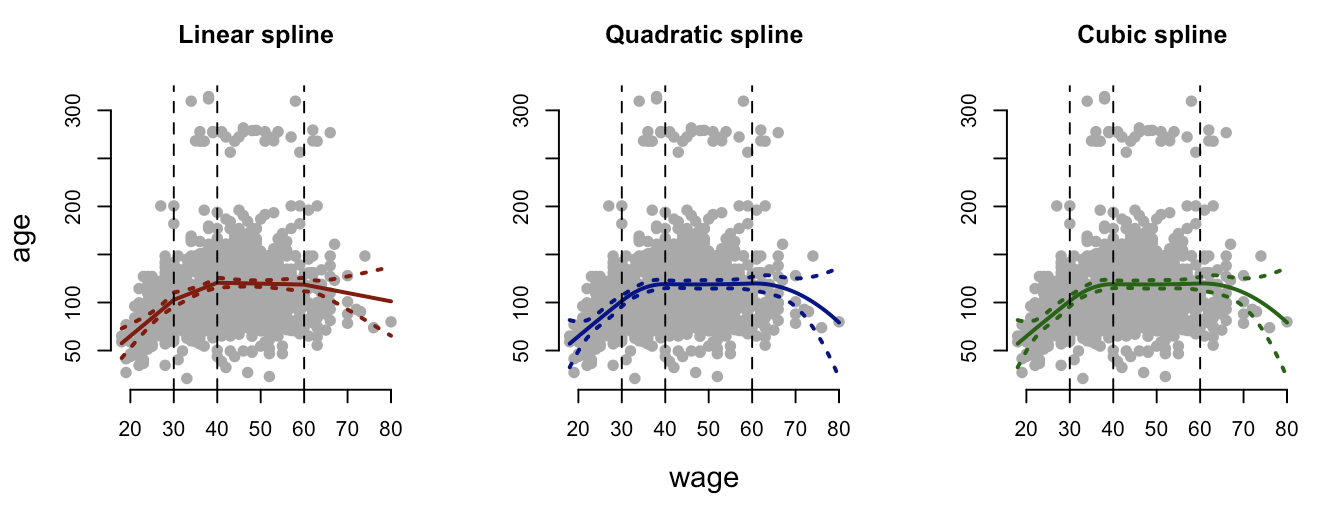
\includegraphics[width=10cm]{images/cubic_splines_issue.png}
\end{frame}
%------------------------------------------------
\begin{frame}{Natural (restricted) cubic spline}
    \begin{itemize}
        \item \alertblue{Natural cubic spline}: cubic spline with \alertblue{additional boundary constraints, enforcing linearity beyond boundary knots} 
        \item Produce more \alertblue{stable estimates at boundaries (narrower confidence intervals)} than cubic splines
    \end{itemize}
    \centering
    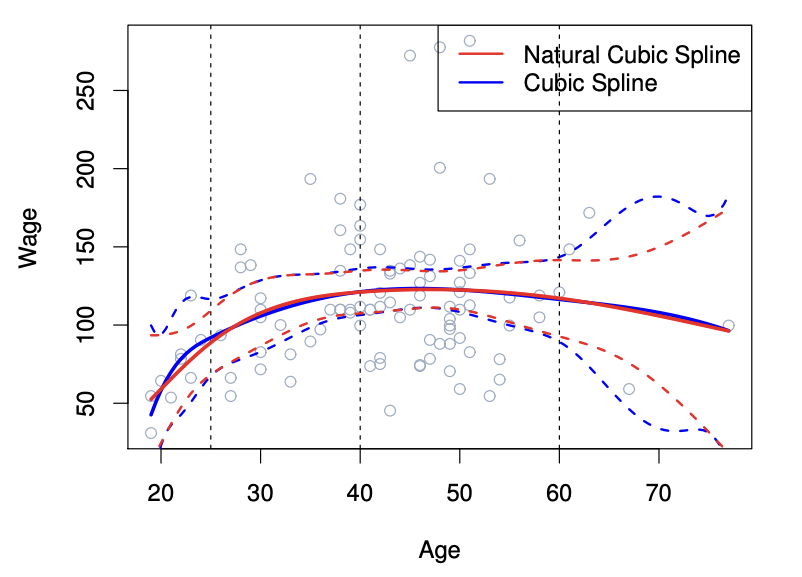
\includegraphics[width=6cm]{images/cubic_vs_natural.png}
    \begin{itemize}
        \item \textbf{\alertblue{How are these concepts used in DLNMs?}}
    \end{itemize}
\end{frame}
%------------------------------------------------
% \begin{frame}{Natural (Restricted) Cubic Spline}
%     \begin{itemize}
%         \item Ensures linearity beyond the boundary by \alertblue{enforcing the second derivative of cubic splines to be zero at the boundary knots}
%         \begin{equation*}
%             \alertblue{\left. \frac{d^2 f}{d x^2} \right|_{x<\xi_1}} = 0, \quad
%             \alertblue{\left. \frac{d^2 f}{d x^2} \right|_{x_n>\xi_k}} = 0
%         \end{equation*}
%         \item Use lower-degree (\alertblue{3}) polynomials making them more flexible (\alertblue{less wiggles and overfitting}) and therefore \alertblue{computationally efficient}
%         \item Splines provide a transparent and interpretable fit (\alertblue{linear in coefficients with non-linear function of predictors})
%         \vspace{0.5cm}
%         \item \textbf{\alertblue{How are these concepts used in DLNMs?}}
%     \end{itemize}
% \end{frame}
%------------------------------------------------
\section{Concept}
\begin{frame}{DLNMs: Conceptual model}
\begin{figure}
    \centering
    \begin{minipage}{0.2\linewidth}
        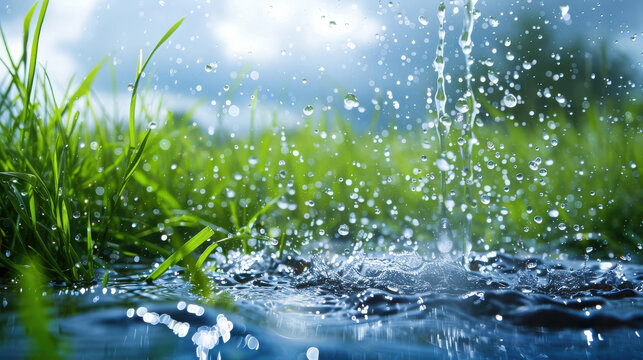
\includegraphics[width=\linewidth]{images/rainfall.jpg}
        \caption{\footnotesize Heavy rainfall \textbf{(Exposure)}}
    \end{minipage}
    \hspace{0.5cm}
    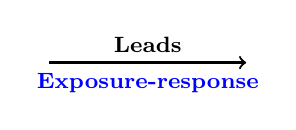
\begin{tikzpicture}
        \draw[->, thick] (0,0) -- (2.5,0) node[midway, above] {\footnotesize \textbf{Leads}} node[midway, below] {\footnotesize \textbf{{\alertblue{Exposure-response}}}};
    \end{tikzpicture}
    \hspace{0.5cm}
    \begin{minipage}{0.2\linewidth}
        \centering
        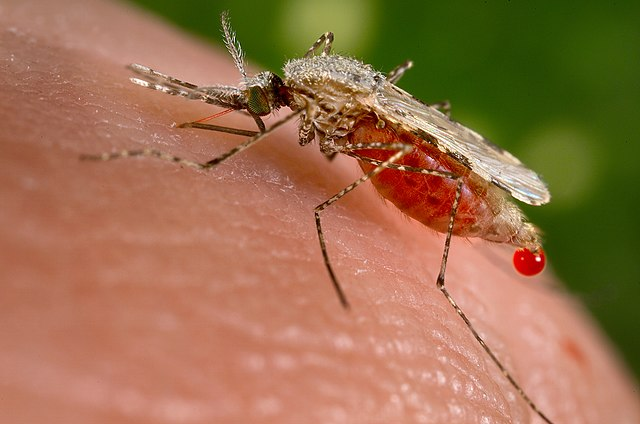
\includegraphics[width=\linewidth]{images/malaria.jpeg}
        \caption{\footnotesize Malaria cases \textbf{(Response)}}
    \end{minipage}
\end{figure}
%------------------------------------------------
\begin{figure}
    \centering
    \begin{minipage}{0.2\linewidth}
        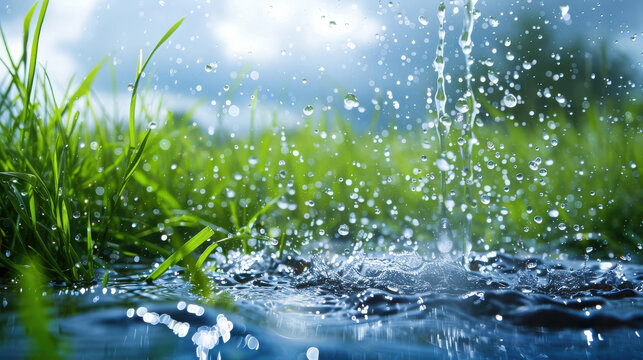
\includegraphics[width=\linewidth]{images/rainfall.jpg}
        \caption{\footnotesize Heavy rainfall \textbf{(Exposure)}}
    \end{minipage}
    \hspace{0.5cm}
    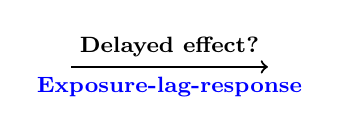
\begin{tikzpicture}
        \draw[->, thick] (0,0) -- (2.5,0) node[midway, above] {\footnotesize \textbf{\alert{Delayed effect?}}} node[midway, below] {\footnotesize \textbf{{\alertblue{Exposure-lag-response}}}};
    \end{tikzpicture}
    \hspace{0.5cm}
    \begin{minipage}{0.2\linewidth}
        \centering
        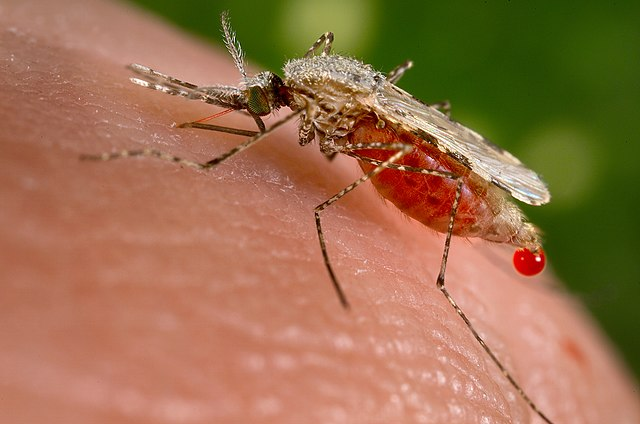
\includegraphics[width=\linewidth]{images/malaria.jpeg}
        \caption{\footnotesize Malaria cases \textbf{(Response)}}
    \end{minipage}
\end{figure}
\end{frame}
%------------------------------------------------
\begin{frame}{DLNMs: Conceptual model}
    \begin{itemize}
        \item DLNMs capture a detailed representation of the \alertblue{time-course} of the \alertblue{exposure-\textbf{lag}-response relationship} 
         \item Risk associated with individual exposure events at each lag \alertblue{assigned a weight} that contributes to \alertblue{overall cumulative risk}
  \end{itemize}  
    \centering
    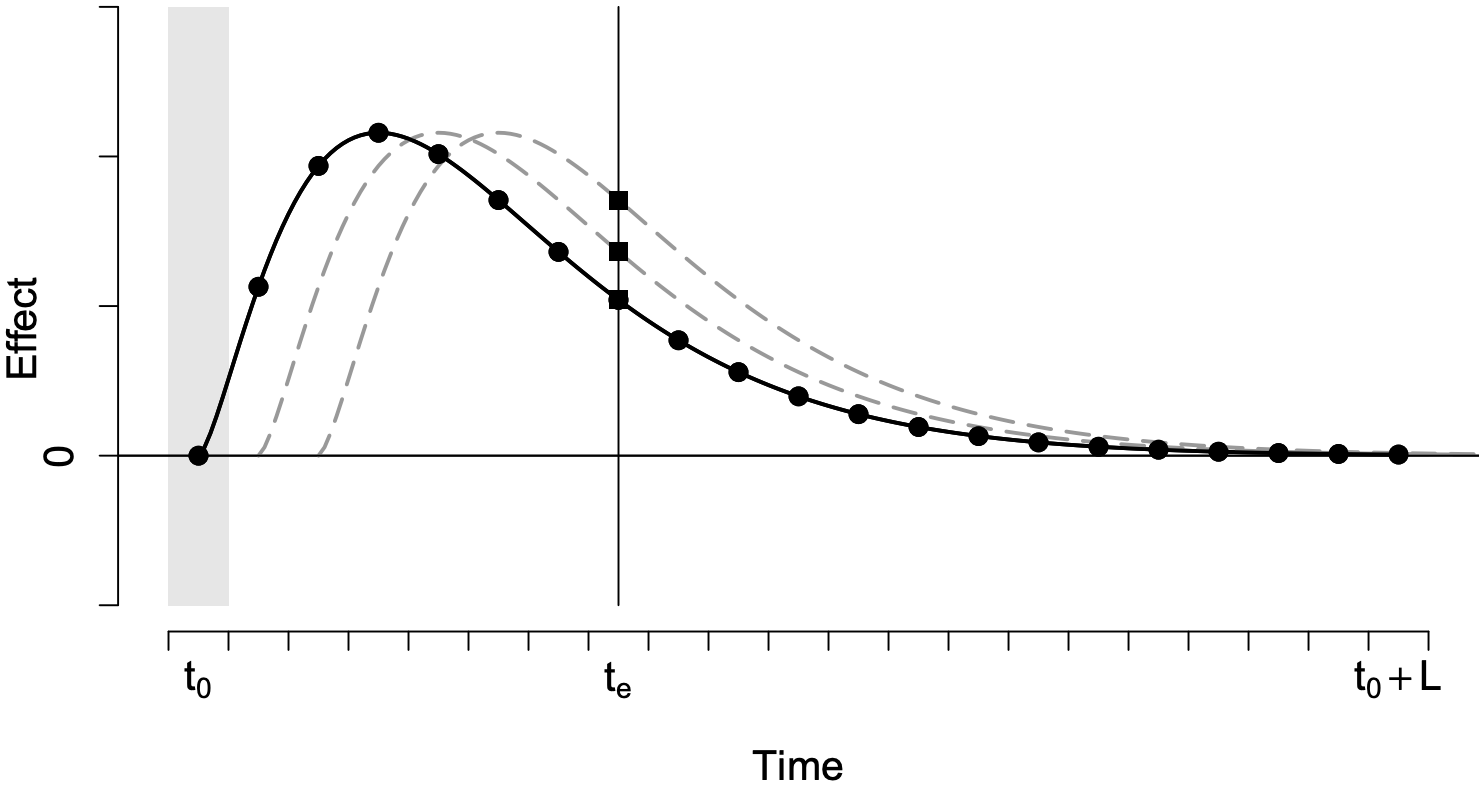
\includegraphics[width=7.5cm,keepaspectratio]{images/delayed effect.png}
  \begin{itemize}
      \item \textbf{\alertblue{Statistical issue is to model this risk!}}
  \end{itemize} 
\end{frame}
%------------------------------------------------
\begin{frame}{Exposure-lag-response associations }
    \begin{itemize}
        \item The risk is represented by a function \alertblue{$s(x, t)$} defined in terms of both \textbf{\alertblue{intensity}} and \textbf{\alertblue{timing}} of a series of \textbf{\alertblue{past exposures}}:
        \vspace{0.1cm}
        \begin{itemize}
            \item an \textbf{\alertblue{exposure-response}} function \alertblue{$f(x)$} for \textbf{\alertblue{exposure $x$}}
            \item a \textbf{\alertblue{lag-response}} function \alertblue{$w(\ell)$} for \textbf{\alertblue{lag $\ell$}}
        \end{itemize}
        \vspace{0.1cm}
        \item Generating a \textbf{\alertblue{bi-dimensional exposure-lag-response}} function 
        \alertblue{\( f \cdot w(\bm{x}, \ell) \)}: \\
        \[
        s(x, t) = \int_{\ell_0}^{L} f(x_{t-\ell}) \cdot w(\ell) \, d\ell \] \\
        \end{itemize}
    \begin{itemize}
        \item Approximation obtained through a \textbf{\alertblue{discretization of the lag period into equally spaced time units}}
    \end{itemize}
        \[
        s(x_{t-\ell_0}, \dots, x_{t-L}) \approx \sum_{\ell = \ell_0}^{L} f(x_{t-\ell}) \cdot w( \ell)
        \]
\end{frame}
%------------------------------------------------
\section{Stats}
\begin{frame}{Basic model}
\begin{itemize}
    \item A general statistical model representation to describe the \alertblue{time series of outcomes \( Y_t \)} with \alertblue{\( t = 1, \dots, n \)} is given by
\end{itemize}
\vspace{0.8cm}
\begin{equation*}
    \eqnmark[blue]{node1}{g(\mu_t)} =
    \eqnmark[red]{node2}{\alpha} +
    \sum_{j=1}^{J} \eqnmarkbox[purple]{node3}{s_j(x_{tj}; \beta_j)} +
    \sum_{k=1}^{K} \eqnmarkbox[brown]{node4}{\gamma_k u_{tk}}
\end{equation*}
    \annotate[yshift=1.2em]{above, left}{node1}{Link function}
    \annotate[yshift=1.2em]{above, right}{node3}{Smoothed predictor}
    \annotate[yshift=-1.2em]{below, left}{node4}{Other predictors with linear effects}
\vspace{0.5cm}
\begin{itemize}
    \item where \alertblue{\( \mu \equiv E(Y) \)}, and \( Y \) is assumed to arise from a distribution belonging to the exponential family  
    \item \alertblue{\(x_{tj}\)} is the transformed exposure at time \alertblue{\(t\)} through basis function \alertblue{\(j\)}
    \item \alertblue{\(\beta_j\)} is unknown coefficient of \alertblue{\(x_{tj}\)} to be estimated
\end{itemize}
\end{frame}
%------------------------------------------------
\begin{frame}{Distributed lag models (DLMs)}
\begin{itemize}
    \item Response \alertblue{\(Y\)} at a given time \alertblue{\(t\)}, (\alertblue{\(Y_t\)}),  may be explained in terms of \textbf{\alertblue{past exposures \( x_{t-\ell} \)}} with \(\ell\) for lags \( \ell = \ell_0, \ldots, \ell, \ldots, L \):
    \[q_{x_t} = [x_{t - \ell_0}, \ldots, x_{t - \ell}, \ldots, x_{t - L}]\]

    \item Assuming a \textbf{\alertblue{linear exposure-response relationship}}, hence \textbf{\alertblue{DLM}}:
    \[s(x,t; \beta) =\sum_{\ell = \ell_0}^{L} x_{t-\ell} \cdot w( \ell)
        \Rightarrow (q_{x_t} C) \beta = w_{x_t} \beta\] 

    \item \textbf{\alertblue{\( C \)}} is obtained by applying a \textbf{\alertblue{specific basis transformation}} \\
    to the lag vector \( \ell = [\ell_0, \ldots, \ell, \ldots, L] \) 
\end{itemize}
\end{frame}
%------------------------------------------------
\begin{frame}{Distributed lag non-linear models (DLNMs)}
\begin{itemize}
    \item \textbf{\alertblue{\( R_{x_t} \)}} is obtained by applying a \textbf{\alertblue{second basis transformation}} to \textbf{\alertblue{\( q_{x_t} \)}}

    \item Then we define a \textbf{\alertblue{special tensor product}}:

\[A_{x_t} = (1_{v_\ell} \otimes R_{x_t}) \odot (C \otimes 1_{v_x})\]

which forms the \textbf{\alertblue{crossbasis}}:

\[s(q_{x_t}; \beta) = (1_{v_x.v_\ell} A_{x_t}) \beta = w_{x_t} \beta\]

    \item \textbf{\alertblue{The problem reduces to choosing a basis function for each \( q_{x_t} \) and \( \ell \)}}, defining \textbf{\alertblue{exposure-response}} and \textbf{\alertblue{lag-response functions}}, respectively
\end{itemize}
\end{frame}
%------------------------------------------------
\section{Crossbasis}
\begin{frame}{Basis for exposure-response function}
    \begin{itemize}
        \item Given, a timeseries of exposure X and assuming a \alertblue{\textbf{maximum lag of 2}},  we can compute, \alertblue{\(q_{xt}\)} (\alertblue{\textbf{vector of lagged exposure histories of X}})
        \item Applying a \alertblue{\textbf{linear transformation}} to \alertblue{\( q_{xt} \) } we get \alertblue{\( R_{xt}\)} \\ (\alertblue{\textbf{lagged occurrences of each of the basis variables of X}})
    \end{itemize}
    \vspace{0.5cm}
\[
\begin{array}{|c|c|}
    t & {x} \\ \hline
    1 & 10  \\
    2 & 20  \\
    3 & 30  \\
    4 & 40  \\
    5 & 50  
\end{array} 
\Rightarrow 
\begin{array}{|c|c|c|c|}
    \fcolorbox{white}{yellow}{lag 0} & \fcolorbox{white}{cyan}{lag 1} & \fcolorbox{white}{lime}{lag 2} \\ \hline
    \fcolorbox{white}{yellow}{10} & \fcolorbox{white}{cyan}{NA} & \fcolorbox{white}{lime}{NA} \\
    \fcolorbox{white}{yellow}{20}  & \fcolorbox{white}{cyan}{10} & \fcolorbox{white}{lime}{NA} \\
    \fcolorbox{white}{yellow}{30}  & \fcolorbox{white}{cyan}{20} & \fcolorbox{white}{lime}{10} \\
    \fcolorbox{white}{yellow}{40}  & \fcolorbox{white}{cyan}{30} & \fcolorbox{white}{lime}{20}  \\
    \fcolorbox{white}{yellow}{50}  & \fcolorbox{white}{cyan}{40} & \fcolorbox{white}{lime}{30} 
\end{array}
\Rightarrow  
\begin{bmatrix}
\fcolorbox{white}{yellow}{10} & \fcolorbox{white}{cyan}{NA} & \fcolorbox{white}{lime}{NA} \\
\fcolorbox{white}{yellow}{20} & \fcolorbox{white}{cyan}{10} & \fcolorbox{white}{lime}{NA} \\
\fcolorbox{white}{yellow}{30} & \fcolorbox{white}{cyan}{20} & \fcolorbox{white}{lime}{10} \\
\fcolorbox{white}{yellow}{40} & \fcolorbox{white}{cyan}{30} & \fcolorbox{white}{lime}{20} \\
\fcolorbox{white}{yellow}{50} & \fcolorbox{white}{cyan}{40} & \fcolorbox{white}{lime}{30} \\
\end{bmatrix}
\]
\end{frame}
%------------------------------------------------
\begin{frame}{Basis for lag-response function}
    \begin{itemize}
        \item Applying \alertblue{\textbf{polynomial transformation of degree 2}} to the lag vector, \(\ell\)(0,1,2)
        \item First step is to scale the lag vector by dividing by the maximum lag:
        \[
        (0,1,2)/2 \Rightarrow (0, 0.5, 1)
        \]
        \item Obtaining \alertblue{C} (\alertblue{\textbf{basis variables for each lag for polynomial degrees d = 0,1,2}})
    \end{itemize}
    \vspace{0.5cm}
\[
\begin{array}{|c|c|c|c|}
    x^d & x^0 & x^1 & x^2 \\ \hline
    \fcolorbox{white}{pink}{lag 0 (0)} & \fcolorbox{white}{pink}{1}  & \fcolorbox{white}{pink}{0}   & \fcolorbox{white}{pink}{0}   \\
    \fcolorbox{white}{lightgray}{lag 1 (0.5)} & \fcolorbox{white}{lightgray}{1}  & \fcolorbox{white}{lightgray}{0.5} & \fcolorbox{white}{lightgray}{0.25} \\
    \fcolorbox{white}{orange}{lag 2 (1)} & \fcolorbox{white}{orange}{1}  & \fcolorbox{white}{orange}{1}   & \fcolorbox{white}{orange}{1}  
\end{array}
\Rightarrow C = 
\begin{bmatrix}
\fcolorbox{white}{pink}{1} & \fcolorbox{white}{pink}{0} & \fcolorbox{white}{pink}{0} \\
\fcolorbox{white}{lightgray}{1} & \fcolorbox{white}{lightgray}{0.5} & \fcolorbox{white}{lightgray}{0.25} \\
\fcolorbox{white}{orange}{1} & \fcolorbox{white}{orange}{1} & \fcolorbox{white}{orange}{1}
\end{bmatrix}
\]
\end{frame}
%------------------------------------------------
\begin{frame}{Special tensor product}
\begin{equation*}
    \eqnmark{node1}{A_{xt}} =
    (\eqnmark[brown]{node2}{1_{vl}}
    \eqnmark[blue]{node3}{\otimes} 
    \eqnmark{node4}{R_{xt}})
    \eqnmark[purple]{node5}{\odot} 
    (\eqnmark{node6}{C} 
    \eqnmark[blue]{node7}{\otimes} 
    \eqnmark[orange]{node8}{1_{vx}})
\end{equation*}
    \annotate[yshift=0.5em]{above, right}{node3}{Kronecker product (matrix direct product)}
    \annotate[yshift=-0.5em]{below, left}{node5}{Hadamard product (element-wise product)}
\vspace{0.5cm}
\begin{itemize}
    \item \( 1_{vx}\): Vector of 1's of dimensional length of exposure vector
\[
\begin{array}{|c|c|}
    t & x  \\ \hline
    1 & 10 \\
    2 & 20 \\
    3 & 30 \\
    4 & 40 \\
    5 & 50 \\
\end{array}
\Rightarrow 1_{vx} =
\begin{bmatrix}
    1 \\
    1 \\
    1 \\
    1 \\
    1 \\
\end{bmatrix}
\]
    \item \( 1_{v\ell}\): Vector of 1's of dimensional length of lag vector
\[ \ell(0,1,2) \Rightarrow 1_{v\ell} =  [1,1,1] \]
\end{itemize}
\end{frame}
%------------------------------------------------
\begin{frame}{\(1_{v\ell} \otimes R_{xt}\)}
\footnotesize
\[
[1,1,1] \otimes
\begin{bmatrix}
\fcolorbox{white}{yellow}{10} & \fcolorbox{white}{cyan}{NA} & \fcolorbox{white}{lime}{NA} \\
\fcolorbox{white}{yellow}{20} & \fcolorbox{white}{cyan}{10} & \fcolorbox{white}{lime}{NA} \\
\fcolorbox{white}{yellow}{30} & \fcolorbox{white}{cyan}{20} & \fcolorbox{white}{lime}{10} \\
\fcolorbox{white}{yellow}{40} & \fcolorbox{white}{cyan}{30} & \fcolorbox{white}{lime}{20} \\
\fcolorbox{white}{yellow}{50} & \fcolorbox{white}{cyan}{40} & \fcolorbox{white}{lime}{30} \\
\end{bmatrix} 
=
\begin{bmatrix} 
\fcolorbox{white}{yellow}{10} & \fcolorbox{white}{yellow}{10} & \fcolorbox{white}{yellow}{10} \\ 
\fcolorbox{white}{yellow}{20} & \fcolorbox{white}{yellow}{20} & \fcolorbox{white}{yellow}{20} \\ 
\fcolorbox{white}{yellow}{30} & \fcolorbox{white}{yellow}{30} & \fcolorbox{white}{yellow}{30} \\ 
\fcolorbox{white}{yellow}{40} & \fcolorbox{white}{yellow}{40} & \fcolorbox{white}{yellow}{40} \\ 
\fcolorbox{white}{yellow}{50} & \fcolorbox{white}{yellow}{50} & \fcolorbox{white}{yellow}{50} \\ 
\fcolorbox{white}{cyan}{NA} & \fcolorbox{white}{cyan}{NA} & \fcolorbox{white}{cyan}{NA} \\
\fcolorbox{white}{cyan}{10} & \fcolorbox{white}{cyan}{10} & \fcolorbox{white}{cyan}{10} \\
\fcolorbox{white}{cyan}{20} & \fcolorbox{white}{cyan}{20} & \fcolorbox{white}{cyan}{20} \\
\fcolorbox{white}{cyan}{30} & \fcolorbox{white}{cyan}{30} & \fcolorbox{white}{cyan}{30} \\
\fcolorbox{white}{cyan}{40} & \fcolorbox{white}{cyan}{40} & \fcolorbox{white}{cyan}{40} \\ 
\fcolorbox{white}{lime}{NA} & \fcolorbox{white}{lime}{NA} & \fcolorbox{white}{lime}{NA} \\
\fcolorbox{white}{lime}{NA} & \fcolorbox{white}{lime}{NA} & \fcolorbox{white}{lime}{NA} \\
\fcolorbox{white}{lime}{10} & \fcolorbox{white}{lime}{10} & \fcolorbox{white}{lime}{10} \\
\fcolorbox{white}{lime}{20} & \fcolorbox{white}{lime}{20} & \fcolorbox{white}{lime}{20} \\
\fcolorbox{white}{lime}{30} & \fcolorbox{white}{lime}{30} & \fcolorbox{white}{lime}{30} \\
\end{bmatrix}
\]
\end{frame}
%------------------------------------------------
\begin{frame}{\(C \otimes 1_{vx}\)}
\footnotesize
\[ 
\begin{bmatrix}
\fcolorbox{white}{pink}{1} & \fcolorbox{white}{pink}{0} & \fcolorbox{white}{pink}{0} \\
\fcolorbox{white}{lightgray}{1} & \fcolorbox{white}{lightgray}{0.5} & \fcolorbox{white}{lightgray}{0.25} \\
\fcolorbox{white}{orange}{1} & \fcolorbox{white}{orange}{1} & \fcolorbox{white}{orange}{1}
\end{bmatrix} \otimes \begin{bmatrix}
    1 \\
    1 \\
    1 \\
    1 \\
    1
\end{bmatrix}
=\begin{bmatrix}
\fcolorbox{white}{pink}{1} & \fcolorbox{white}{pink}{0} & \fcolorbox{white}{pink}{0} \\
\fcolorbox{white}{pink}{1} & \fcolorbox{white}{pink}{0} & \fcolorbox{white}{pink}{0} \\
\fcolorbox{white}{pink}{1} & \fcolorbox{white}{pink}{0} & \fcolorbox{white}{pink}{0} \\
\fcolorbox{white}{pink}{1} & \fcolorbox{white}{pink}{0} & \fcolorbox{white}{pink}{0} \\
\fcolorbox{white}{pink}{1} & \fcolorbox{white}{pink}{0} & \fcolorbox{white}{pink}{0} \\
\fcolorbox{white}{lightgray}{1} & \fcolorbox{white}{lightgray}{0.5} & \fcolorbox{white}{lightgray}{0.25} \\
\fcolorbox{white}{lightgray}{1} & \fcolorbox{white}{lightgray}{0.5} & \fcolorbox{white}{lightgray}{0.25} \\
\fcolorbox{white}{lightgray}{1} & \fcolorbox{white}{lightgray}{0.5} & \fcolorbox{white}{lightgray}{0.25} \\
\fcolorbox{white}{lightgray}{1} & \fcolorbox{white}{lightgray}{0.5} & \fcolorbox{white}{lightgray}{0.25} \\
\fcolorbox{white}{lightgray}{1} & \fcolorbox{white}{lightgray}{0.5} & \fcolorbox{white}{lightgray}{0.25} \\
\fcolorbox{white}{orange}{1} & \fcolorbox{white}{orange}{1} & \fcolorbox{white}{orange}{1} \\
\fcolorbox{white}{orange}{1} & \fcolorbox{white}{orange}{1} & \fcolorbox{white}{orange}{1} \\
\fcolorbox{white}{orange}{1} & \fcolorbox{white}{orange}{1} & \fcolorbox{white}{orange}{1} \\
\fcolorbox{white}{orange}{1} & \fcolorbox{white}{orange}{1} & \fcolorbox{white}{orange}{1} \\
\fcolorbox{white}{orange}{1} & \fcolorbox{white}{orange}{1} & \fcolorbox{white}{orange}{1}
\end{bmatrix}
\]
\end{frame}
%------------------------------------------------
\begin{frame}{(\(1_{v\ell} \otimes R_{xt}\)) \(\odot\) (\(C \otimes 1_{vx}\)) = $A_{xt}$}
\footnotesize
\[
\begin{bmatrix} 
\fcolorbox{white}{yellow}{10} & \fcolorbox{white}{yellow}{10} & \fcolorbox{white}{yellow}{10} \\ 
\fcolorbox{white}{yellow}{20} & \fcolorbox{white}{yellow}{20} & \fcolorbox{white}{yellow}{20} \\ 
\fcolorbox{white}{yellow}{30} & \fcolorbox{white}{yellow}{30} & \fcolorbox{white}{yellow}{30} \\ 
\fcolorbox{white}{yellow}{40} & \fcolorbox{white}{yellow}{40} & \fcolorbox{white}{yellow}{40} \\ 
\fcolorbox{white}{yellow}{50} & \fcolorbox{white}{yellow}{50} & \fcolorbox{white}{yellow}{50} \\ 
\fcolorbox{white}{cyan}{NA} & \fcolorbox{white}{cyan}{NA} & \fcolorbox{white}{cyan}{NA} \\
\fcolorbox{white}{cyan}{10} & \fcolorbox{white}{cyan}{10} & \fcolorbox{white}{cyan}{10} \\
\fcolorbox{white}{cyan}{20} & \fcolorbox{white}{cyan}{20} & \fcolorbox{white}{cyan}{20} \\
\fcolorbox{white}{cyan}{30} & \fcolorbox{white}{cyan}{30} & \fcolorbox{white}{cyan}{30} \\
\fcolorbox{white}{cyan}{40} & \fcolorbox{white}{cyan}{40} & \fcolorbox{white}{cyan}{40} \\ 
\fcolorbox{white}{lime}{NA} & \fcolorbox{white}{lime}{NA} & \fcolorbox{white}{lime}{NA} \\
\fcolorbox{white}{lime}{NA} & \fcolorbox{white}{lime}{NA} & \fcolorbox{white}{lime}{NA} \\
\fcolorbox{white}{lime}{10} & \fcolorbox{white}{lime}{10} & \fcolorbox{white}{lime}{10} \\
\fcolorbox{white}{lime}{20} & \fcolorbox{white}{lime}{20} & \fcolorbox{white}{lime}{20} \\
\fcolorbox{white}{lime}{30} & \fcolorbox{white}{lime}{30} & \fcolorbox{white}{lime}{30} \\
\end{bmatrix} \odot \begin{bmatrix}
\fcolorbox{white}{pink}{1} & \fcolorbox{white}{pink}{0} & \fcolorbox{white}{pink}{0} \\
\fcolorbox{white}{pink}{1} & \fcolorbox{white}{pink}{0} & \fcolorbox{white}{pink}{0} \\
\fcolorbox{white}{pink}{1} & \fcolorbox{white}{pink}{0} & \fcolorbox{white}{pink}{0} \\
\fcolorbox{white}{pink}{1} & \fcolorbox{white}{pink}{0} & \fcolorbox{white}{pink}{0} \\
\fcolorbox{white}{pink}{1} & \fcolorbox{white}{pink}{0} & \fcolorbox{white}{pink}{0} \\
\fcolorbox{white}{lightgray}{1} & \fcolorbox{white}{lightgray}{0.5} & \fcolorbox{white}{lightgray}{0.25} \\
\fcolorbox{white}{lightgray}{1} & \fcolorbox{white}{lightgray}{0.5} & \fcolorbox{white}{lightgray}{0.25} \\
\fcolorbox{white}{lightgray}{1} & \fcolorbox{white}{lightgray}{0.5} & \fcolorbox{white}{lightgray}{0.25} \\
\fcolorbox{white}{lightgray}{1} & \fcolorbox{white}{lightgray}{0.5} & \fcolorbox{white}{lightgray}{0.25} \\
\fcolorbox{white}{lightgray}{1} & \fcolorbox{white}{lightgray}{0.5} & \fcolorbox{white}{lightgray}{0.25} \\
\fcolorbox{white}{orange}{1} & \fcolorbox{white}{orange}{1} & \fcolorbox{white}{orange}{1} \\
\fcolorbox{white}{orange}{1} & \fcolorbox{white}{orange}{1} & \fcolorbox{white}{orange}{1} \\
\fcolorbox{white}{orange}{1} & \fcolorbox{white}{orange}{1} & \fcolorbox{white}{orange}{1} \\
\fcolorbox{white}{orange}{1} & \fcolorbox{white}{orange}{1} & \fcolorbox{white}{orange}{1} \\
\fcolorbox{white}{orange}{1} & \fcolorbox{white}{orange}{1} & \fcolorbox{white}{orange}{1}
\end{bmatrix} = \begin{bmatrix}
\fcolorbox{white}{green}{10} & \fcolorbox{white}{teal}{0} & \fcolorbox{white}{olive}{0} \\
\fcolorbox{white}{green}{20} & \fcolorbox{white}{teal}{0} & \fcolorbox{white}{olive}{0} \\
\fcolorbox{white}{green}{30} & \fcolorbox{white}{teal}{0} & \fcolorbox{white}{olive}{0} \\
\fcolorbox{white}{green}{40} & \fcolorbox{white}{teal}{0} & \fcolorbox{white}{olive}{0} \\ 
\fcolorbox{white}{green}{50} & \fcolorbox{white}{teal}{0} & \fcolorbox{white}{olive}{0} \\ \hdashline
\fcolorbox{white}{green}{NA} & \fcolorbox{white}{teal}{NA} & \fcolorbox{white}{olive}{NA} \\ 
\fcolorbox{white}{green}{10} & \fcolorbox{white}{teal}{5} & \fcolorbox{white}{olive}{2.5} \\
\fcolorbox{white}{green}{20} & \fcolorbox{white}{teal}{10} & \fcolorbox{white}{olive}{5} \\
\fcolorbox{white}{green}{30} & \fcolorbox{white}{teal}{15} & \fcolorbox{white}{olive}{7.5} \\
\fcolorbox{white}{green}{40} & \fcolorbox{white}{teal}{20} & \fcolorbox{white}{olive}{10} \\ \hdashline
\fcolorbox{white}{green}{NA} & \fcolorbox{white}{teal}{NA} & \fcolorbox{white}{olive}{NA} \\
\fcolorbox{white}{green}{NA} & \fcolorbox{white}{teal}{NA} & \fcolorbox{white}{olive}{NA} \\
\fcolorbox{white}{green}{10} & \fcolorbox{white}{teal}{10} & \fcolorbox{white}{olive}{10} \\
\fcolorbox{white}{green}{20} & \fcolorbox{white}{teal}{20} & \fcolorbox{white}{olive}{20} \\
\fcolorbox{white}{green}{30} & \fcolorbox{white}{teal}{30} & \fcolorbox{white}{olive}{30} \\
\end{bmatrix}
\]
\end{frame}
%------------------------------------------------
\begin{frame}{Cumulative risk of exposures across lags}
\begin{itemize}
    \item From Gasparrini et al 2010 "\ldots array \alertblue{\(A_{xt}\)} is then re-arranged \textbf{\alertblue{summing along the third dimension of lags}} to obtain the \alertblue{\textbf{final matrix of cross-basis functions, \(w_{xt}\)}}." 
\end{itemize}
\vspace{0.3cm}
\[
A_{x_t}
\Rightarrow 
\begin{bmatrix}
\fcolorbox{white}{green}{10} & \fcolorbox{white}{teal}{0} & \fcolorbox{white}{olive}{0} \\
\fcolorbox{white}{green}{20} & \fcolorbox{white}{teal}{0} & \fcolorbox{white}{olive}{0} \\
\fcolorbox{white}{green}{30} & \fcolorbox{white}{teal}{0} & \fcolorbox{white}{olive}{0} \\
\fcolorbox{white}{green}{40} & \fcolorbox{white}{teal}{0} & \fcolorbox{white}{olive}{0} \\ 
\fcolorbox{white}{green}{50} & \fcolorbox{white}{teal}{0} & \fcolorbox{white}{olive}{0}
\end{bmatrix} \oplus
\begin{bmatrix}
\fcolorbox{white}{green}{NA} & \fcolorbox{white}{teal}{NA} & \fcolorbox{white}{olive}{NA} \\ 
\fcolorbox{white}{green}{10} & \fcolorbox{white}{teal}{5} & \fcolorbox{white}{olive}{2.5} \\
\fcolorbox{white}{green}{20} & \fcolorbox{white}{teal}{10} & \fcolorbox{white}{olive}{5} \\
\fcolorbox{white}{green}{30} & \fcolorbox{white}{teal}{15} & \fcolorbox{white}{olive}{7.5} \\
\fcolorbox{white}{green}{40} & \fcolorbox{white}{teal}{20} & \fcolorbox{white}{olive}{10}
\end{bmatrix} \oplus
\begin{bmatrix}
\fcolorbox{white}{green}{NA} & \fcolorbox{white}{teal}{NA} & \fcolorbox{white}{olive}{NA} \\
\fcolorbox{white}{green}{NA} & \fcolorbox{white}{teal}{NA} & \fcolorbox{white}{olive}{NA} \\
\fcolorbox{white}{green}{10} & \fcolorbox{white}{teal}{10} & \fcolorbox{white}{olive}{10} \\
\fcolorbox{white}{green}{20} & \fcolorbox{white}{teal}{20} & \fcolorbox{white}{olive}{20} \\
\fcolorbox{white}{green}{30} & \fcolorbox{white}{teal}{30} & \fcolorbox{white}{olive}{30} 
\end{bmatrix}
\]

\[ Direct-sum (\oplus) \Rightarrow
\begin{bmatrix}
\fcolorbox{white}{green}{NA} & \fcolorbox{white}{teal}{NA} & \fcolorbox{white}{olive}{NA} \\
\fcolorbox{white}{green}{NA} & \fcolorbox{white}{teal}{NA} & \fcolorbox{white}{olive}{NA} \\
\fcolorbox{white}{green}{60} & \fcolorbox{white}{teal}{20} & \fcolorbox{white}{olive}{15} \\
\fcolorbox{white}{green}{90} & \fcolorbox{white}{teal}{35} & \fcolorbox{white}{olive}{27.5} \\
\fcolorbox{white}{green}{120} & \fcolorbox{white}{teal}{50} & \fcolorbox{white}{olive}{40} \\
\end{bmatrix} = w_{xt}\beta
\]
\end{frame}
%------------------------------------------------
\begin{frame}{Crossbasis functions}
    \centering
    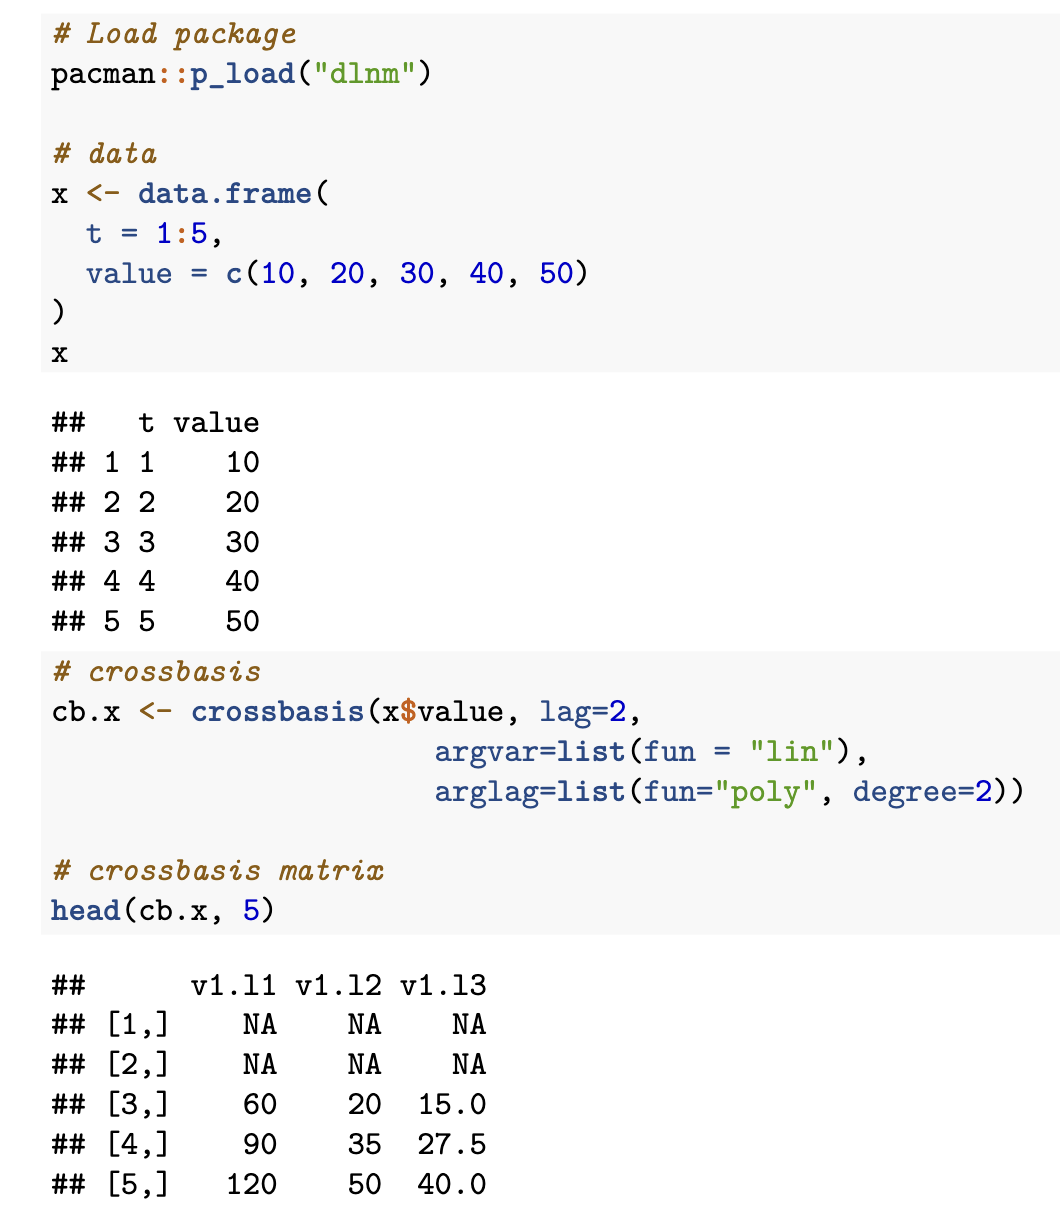
\includegraphics[width=6.25cm,keepaspectratio]{images/crossbasis_result.png}
\end{frame}
%------------------------------------------------
\section{Application}
\begin{frame}{Effect of temperature and ozone on mortality}
\centering
    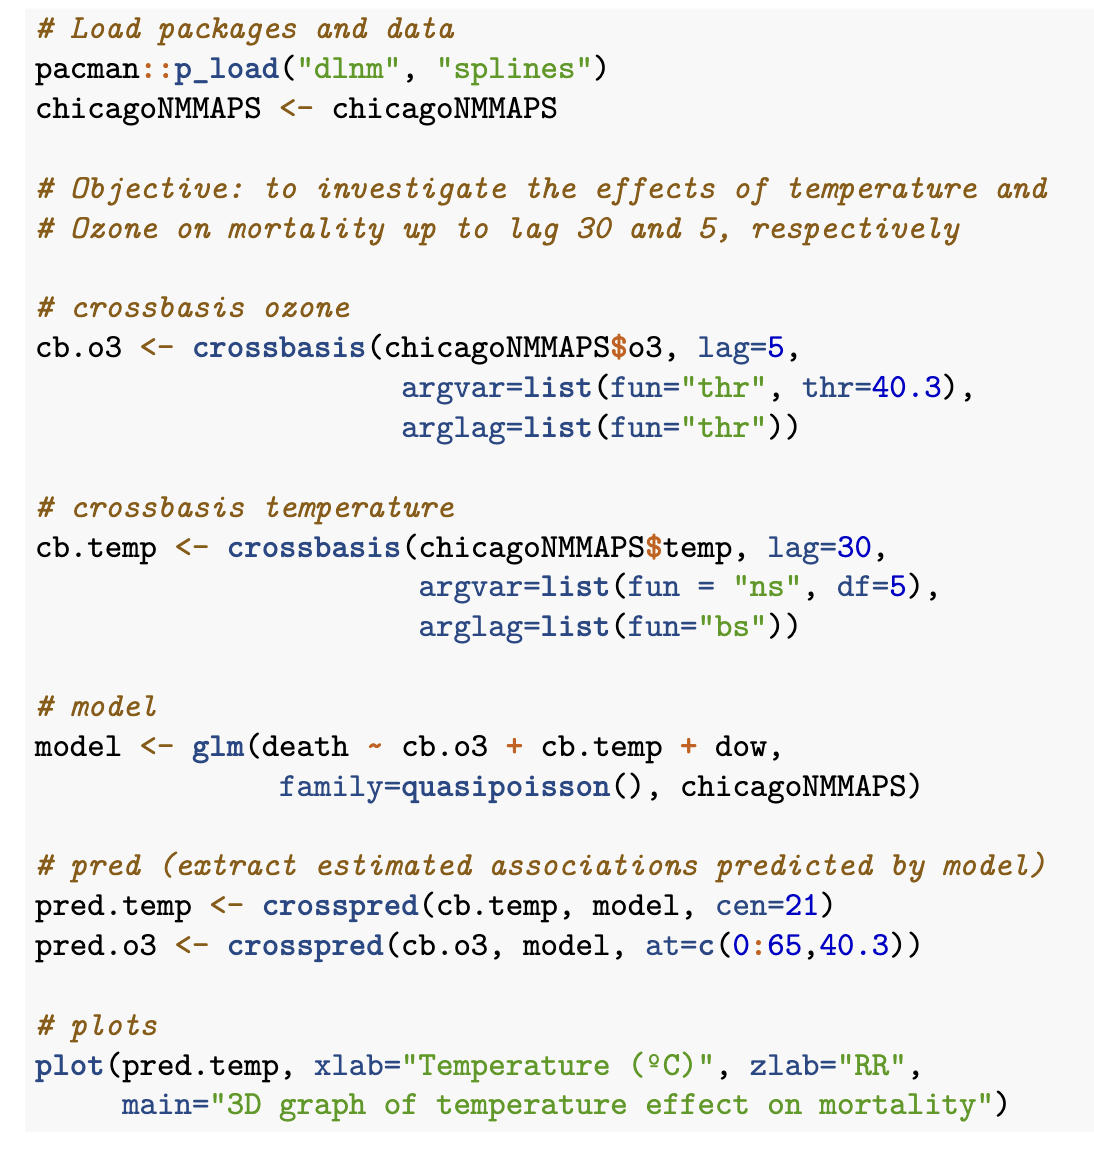
\includegraphics[width=6.83cm,keepaspectratio]{images/code_example_1.png}
\end{frame}
%------------------------------------------------
\begin{frame}{Effect of temperature and ozone on mortality}
\begin{columns}
    \begin{column}{0.6\textwidth}
        \centering
        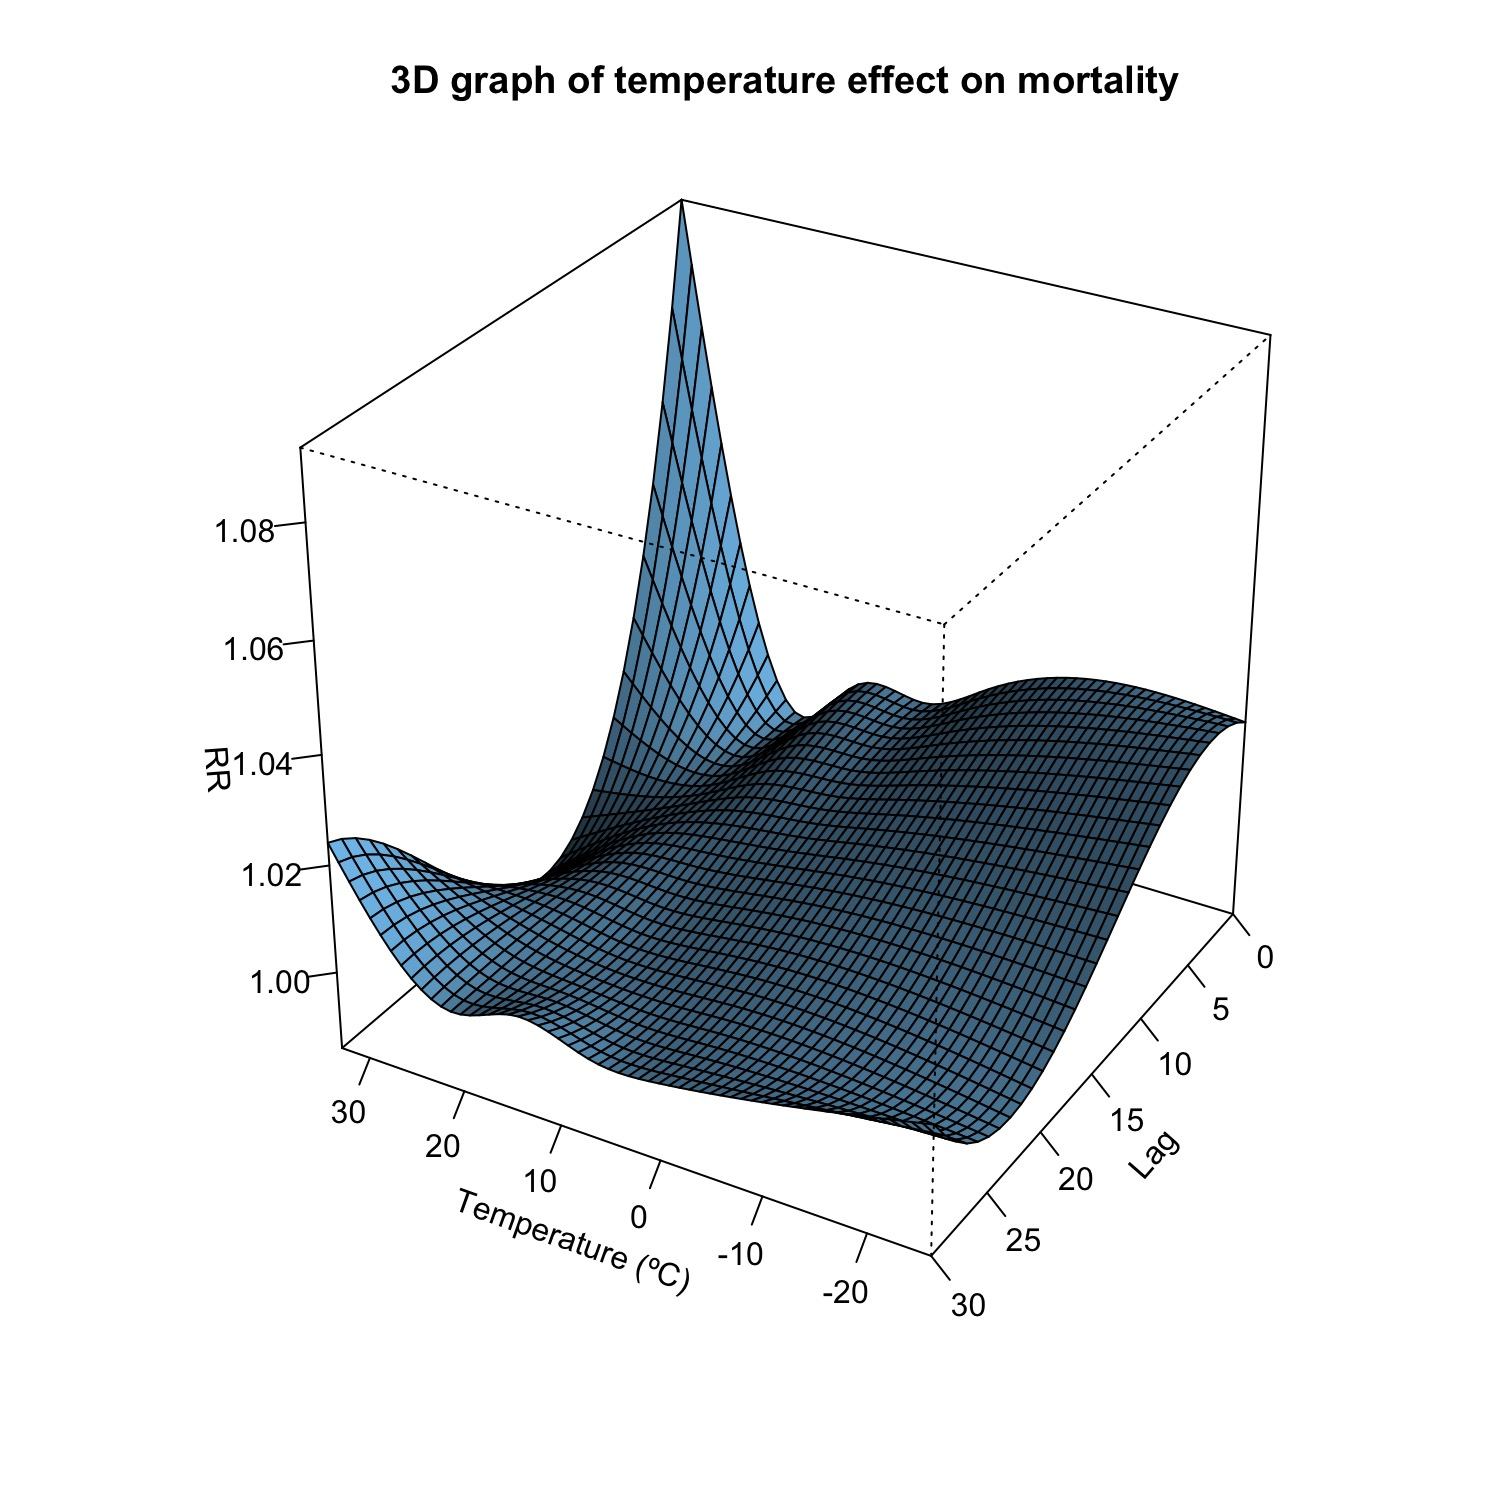
\includegraphics[width=\linewidth]{images/dlnm_example_1.jpeg}
    \end{column}
    \begin{column}{0.6\textwidth}
        \centering
        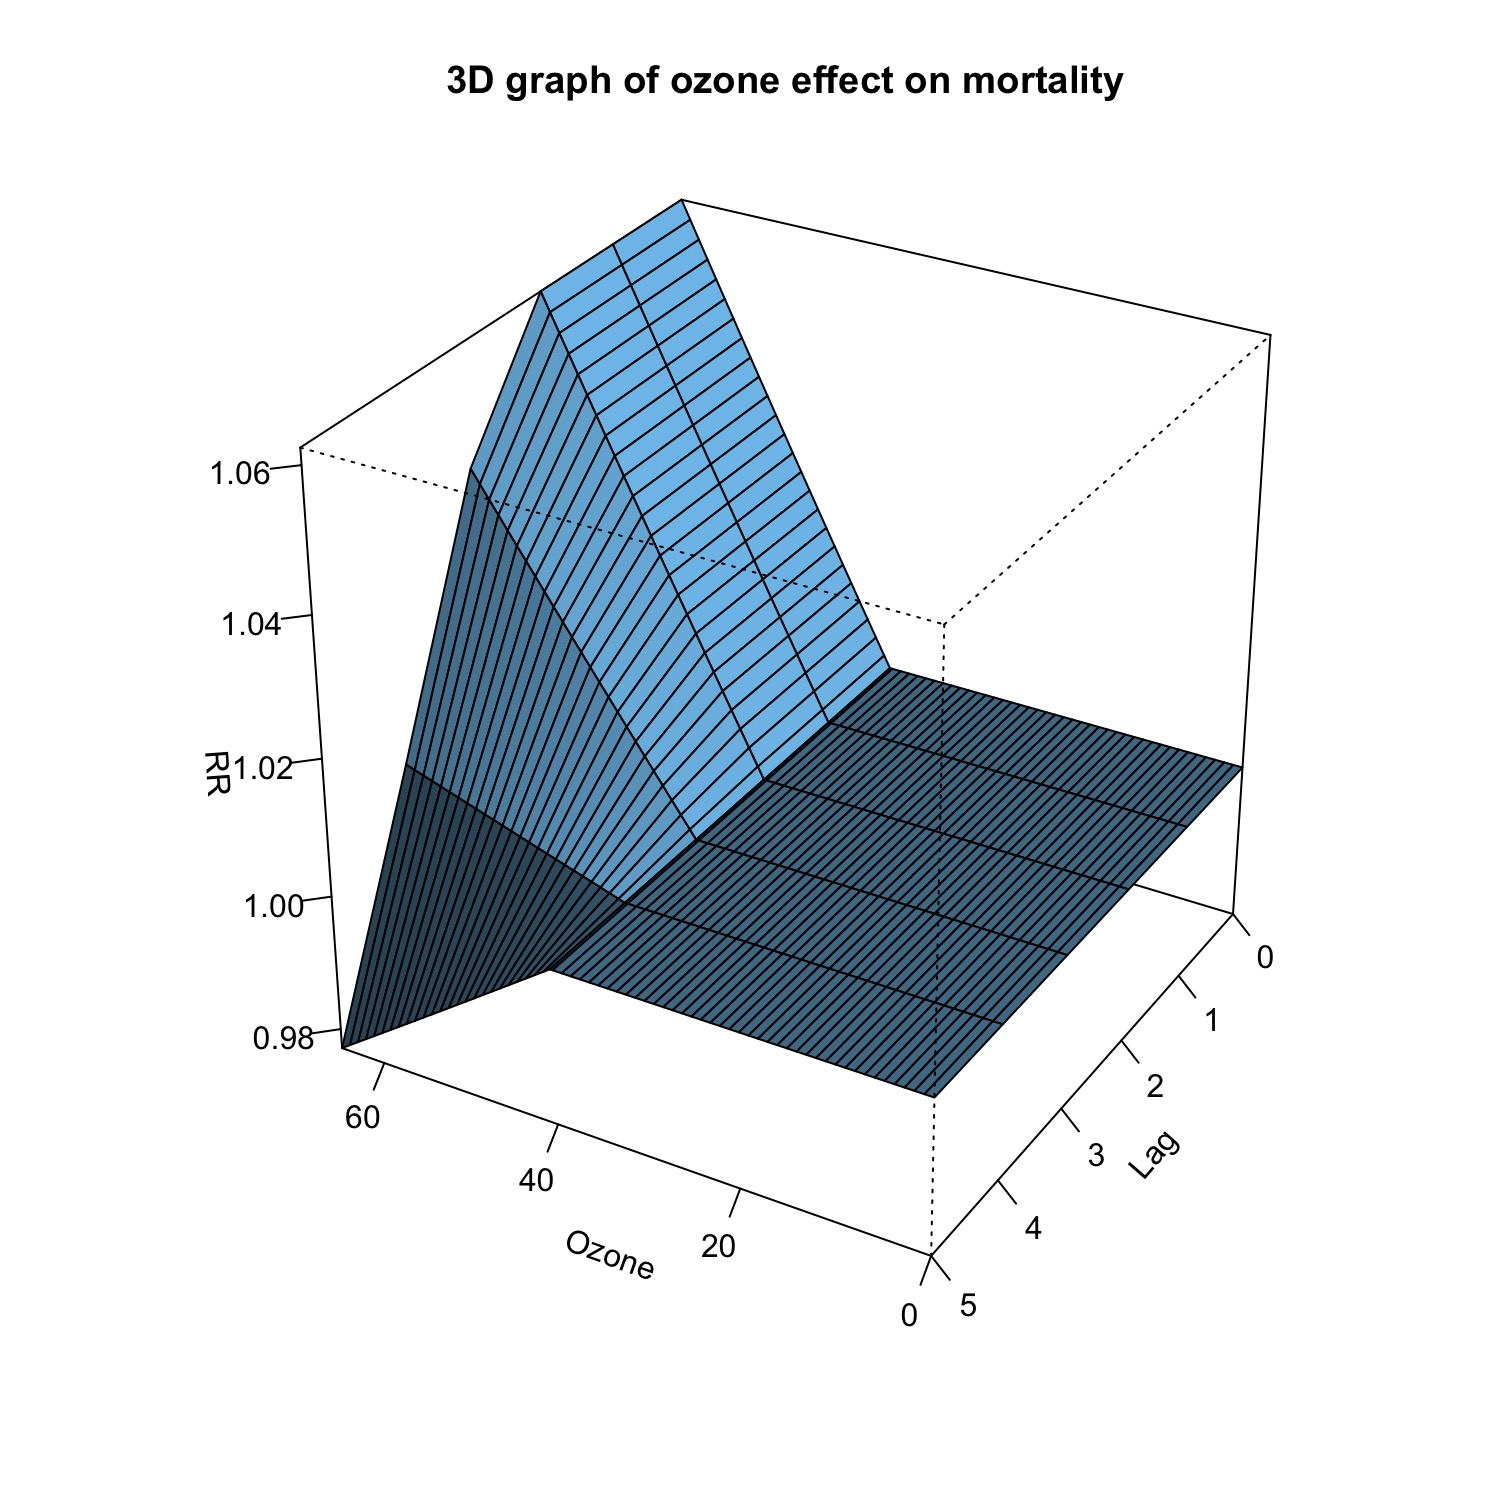
\includegraphics[width=\linewidth]{images/dlnm_example_1_2.jpeg}
    \end{column}
\end{columns}
\end{frame}
%------------------------------------------------
\begin{frame}{Effect of rainfall and temperature on dengue risk}
\centering
    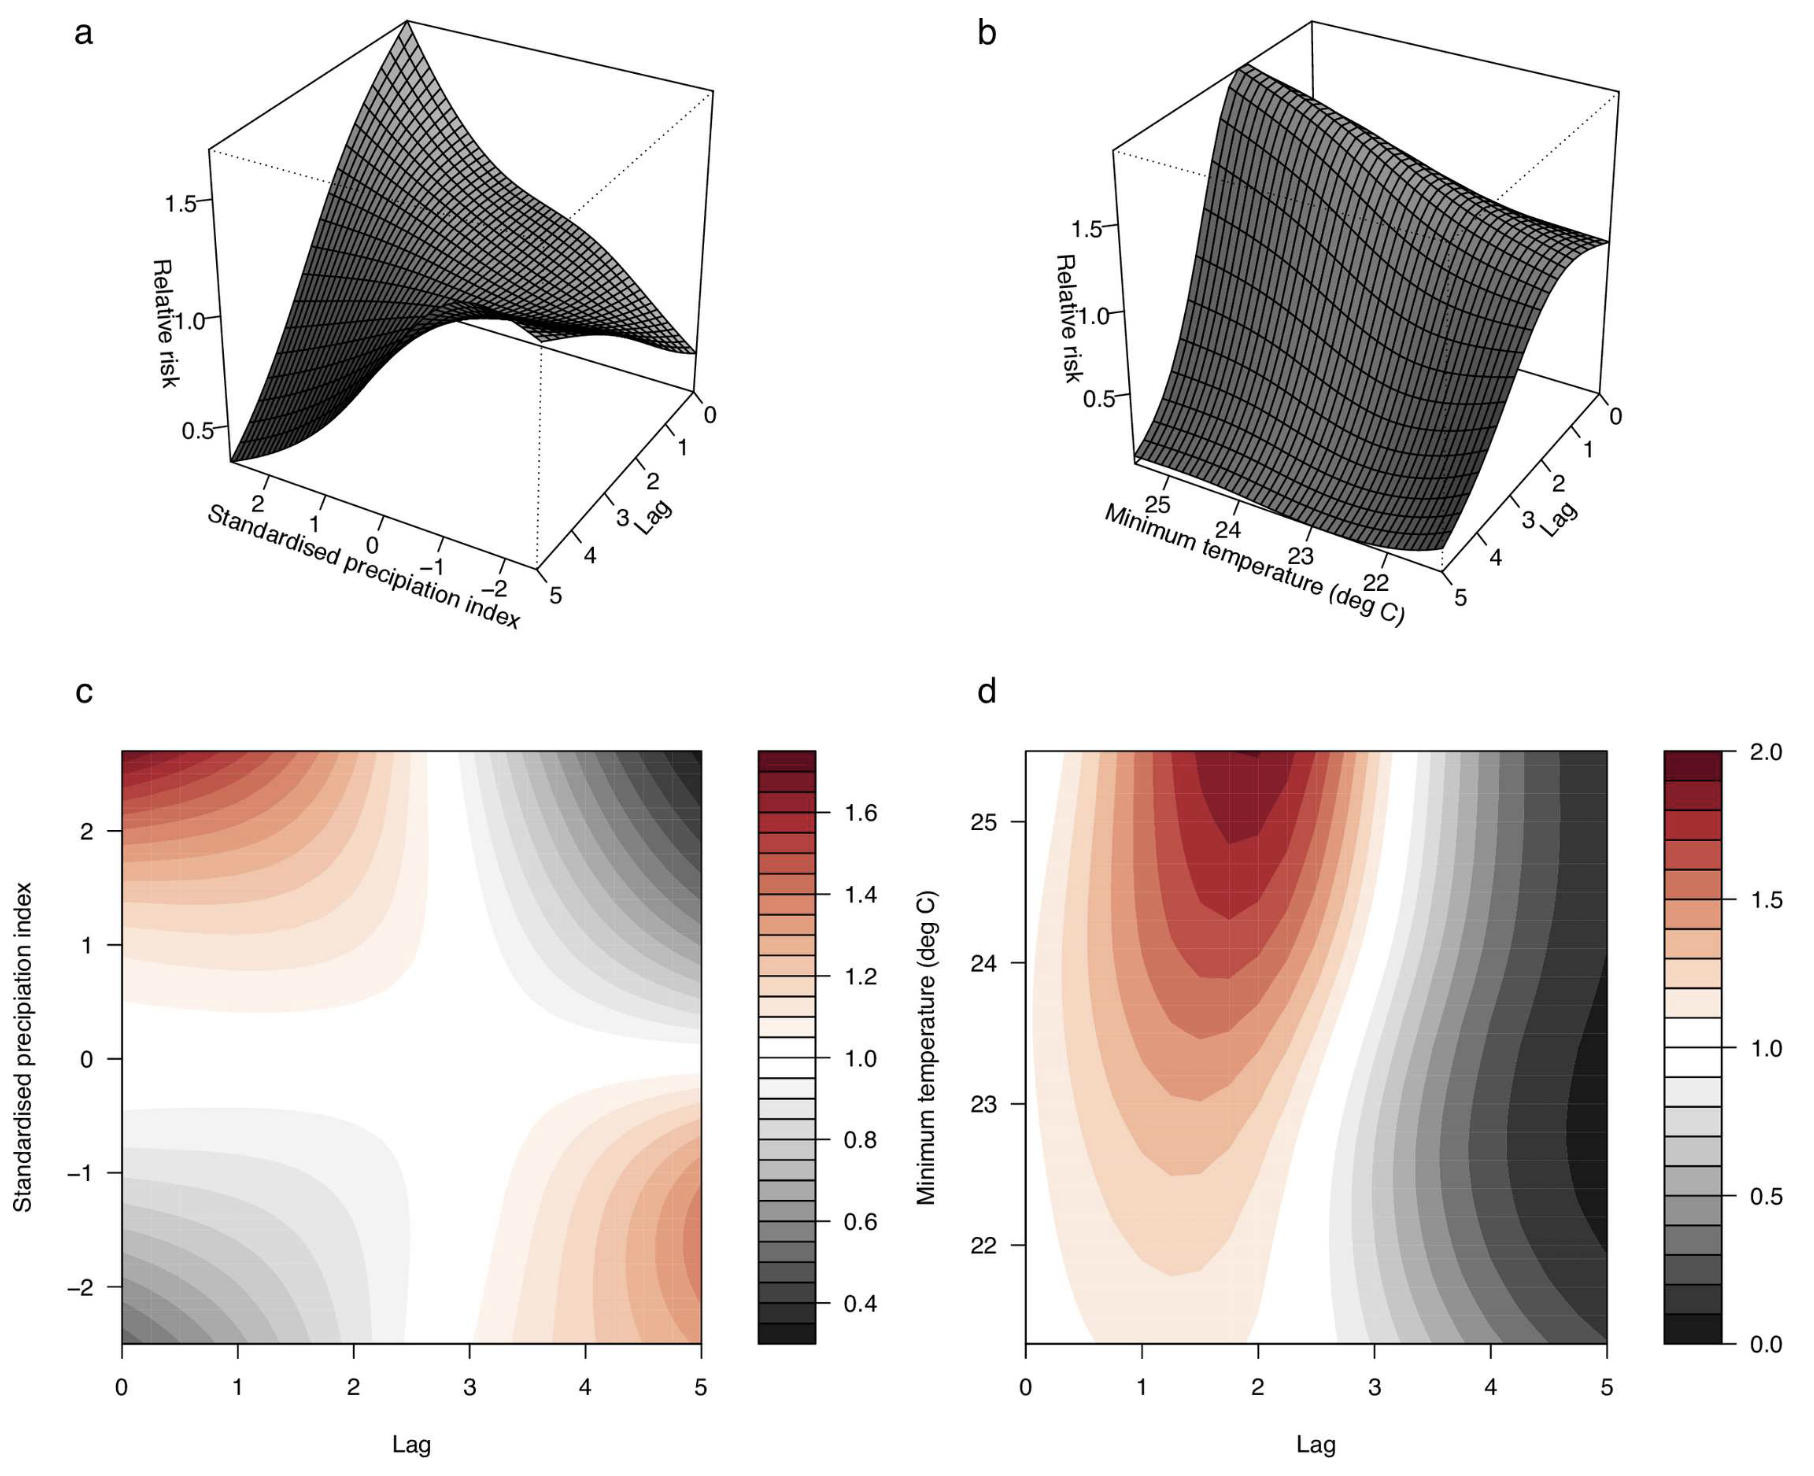
\includegraphics[width=8.8cm,keepaspectratio]{images/dlnm_example_2.png}    
\end{frame}
\begin{frame}{Alternative study designs}
    \centering
    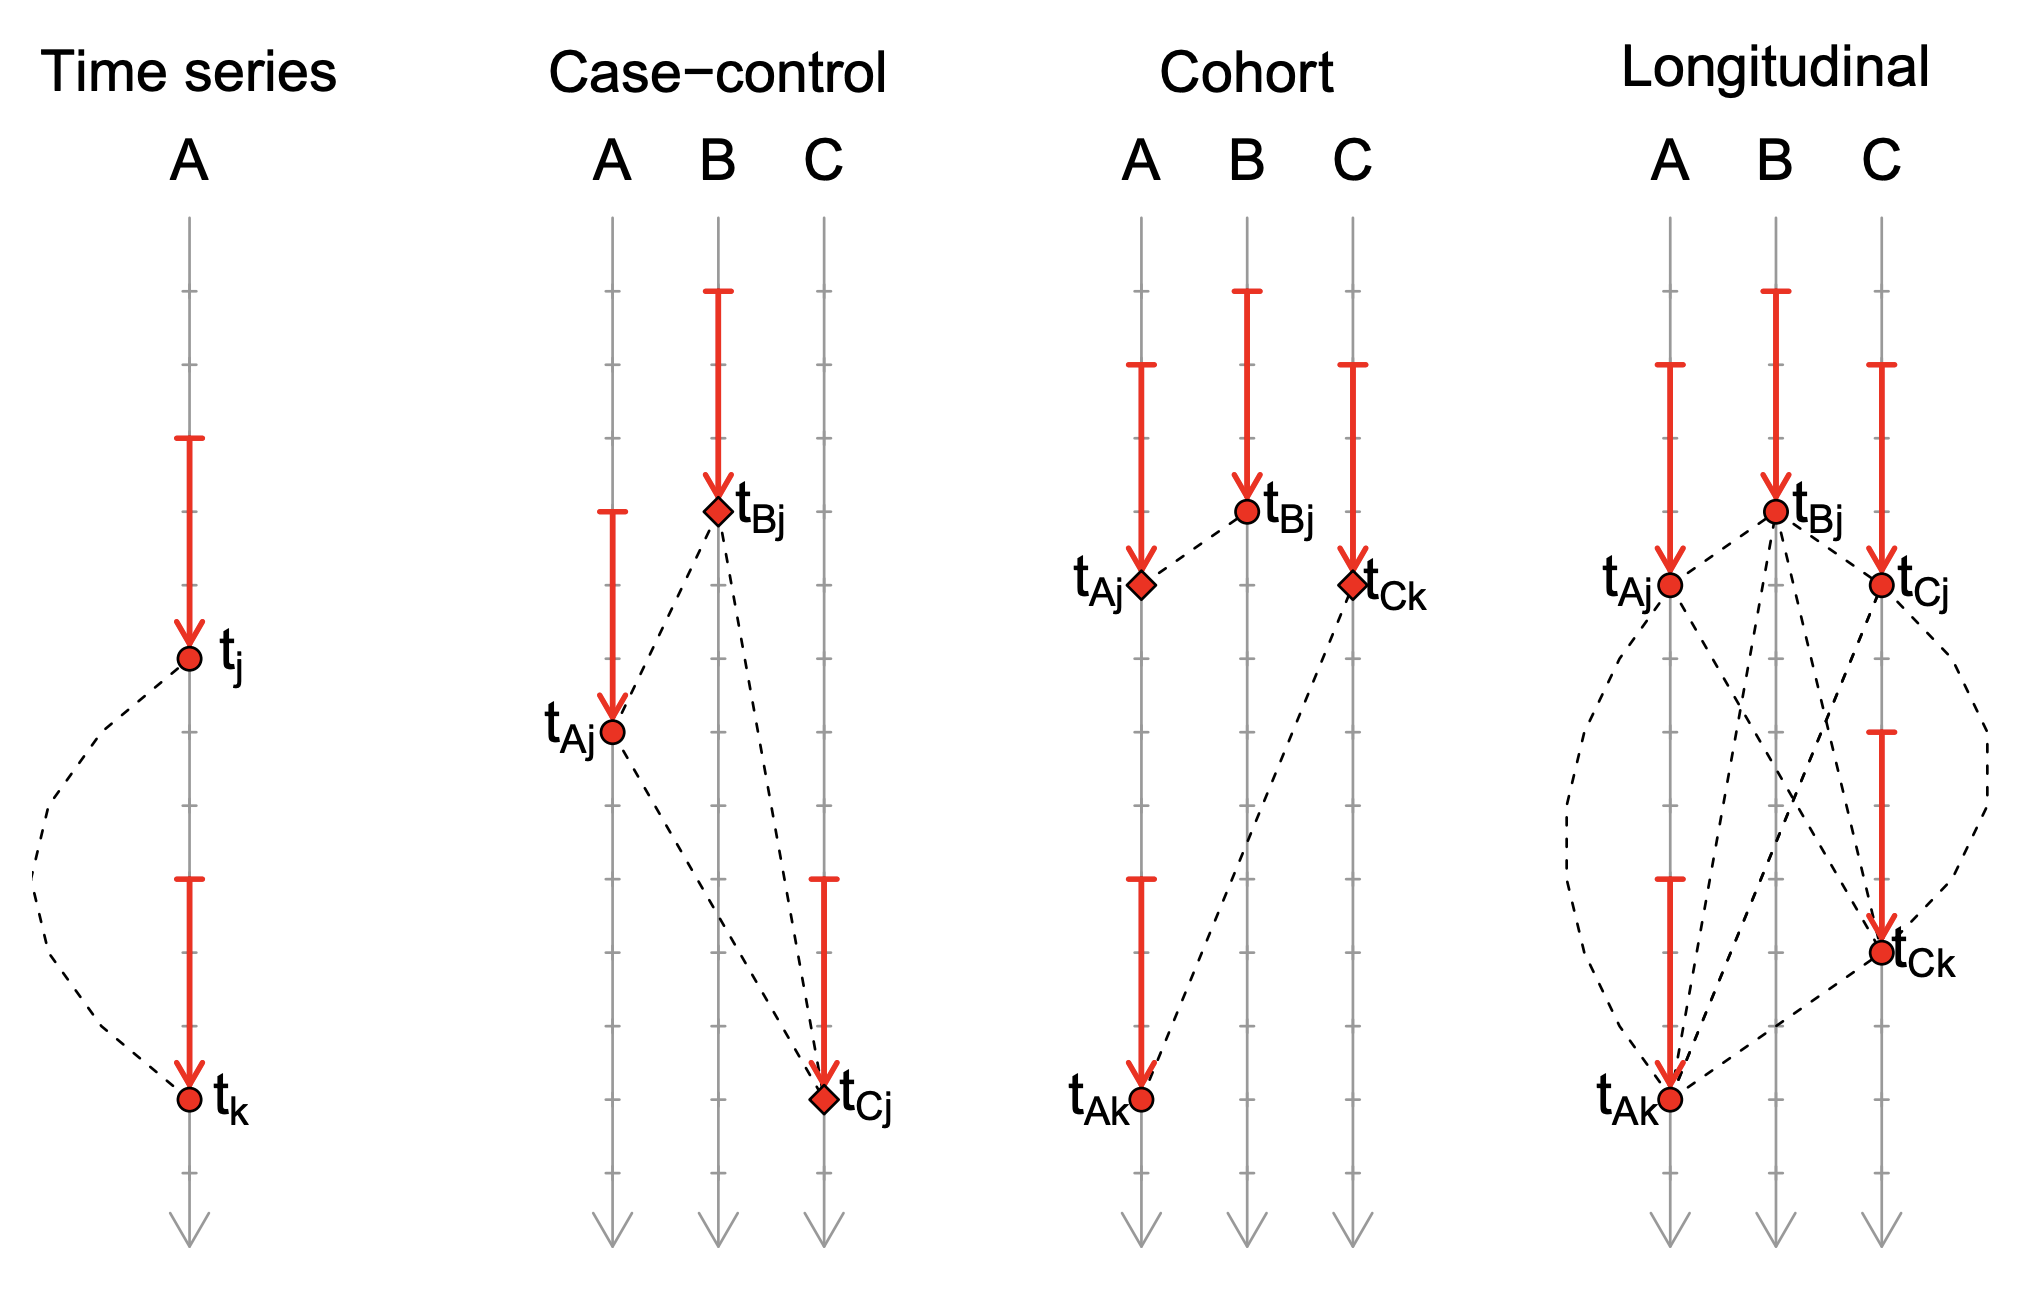
\includegraphics[width=9cm,keepaspectratio]{images/use_cases.png}
\end{frame}
%------------------------------------------------
\begin{frame}{References}
    \begin{itemize}
        \item \cite{gasparrini_distributed_2010}
        \item \cite{gasparrini_distributed_2011}
        \item\cite{gareth_james__daniela_witten__trevor_hastie_introduction_nodate}
        \item \cite{gasparrini_attributable_2014}
        \item \cite{asenmacher_exposure-lag-response_2016}
        \item \cite{lowe_nonlinear_2018}
    \end{itemize}
    \vspace{1em}
    \centering
    \textbf{\large Thank You!} \\
    \vspace{1em}
    Slides: \href{https://github.com/arumadri/dlnm}{\alertblue{https://github.com/arumadri/dlnm}}
\end{frame}
%------------------------------------------------
\end{document}
